% Options for packages loaded elsewhere
\PassOptionsToPackage{unicode}{hyperref}
\PassOptionsToPackage{hyphens}{url}
\documentclass[
  12pt,
  oneside]{book}
\usepackage{xcolor}
\usepackage[left=4cm, right=3cm, top=2.5cm, bottom=2.5cm]{geometry}
\usepackage{amsmath,amssymb}
\setcounter{secnumdepth}{5}
\usepackage{iftex}
\ifPDFTeX
  \usepackage[T1]{fontenc}
  \usepackage[utf8]{inputenc}
  \usepackage{textcomp} % provide euro and other symbols
\else % if luatex or xetex
  \usepackage{unicode-math} % this also loads fontspec
  \defaultfontfeatures{Scale=MatchLowercase}
  \defaultfontfeatures[\rmfamily]{Ligatures=TeX,Scale=1}
\fi
\usepackage{lmodern}
\ifPDFTeX\else
  % xetex/luatex font selection
\fi
% Use upquote if available, for straight quotes in verbatim environments
\IfFileExists{upquote.sty}{\usepackage{upquote}}{}
\IfFileExists{microtype.sty}{% use microtype if available
  \usepackage[]{microtype}
  \UseMicrotypeSet[protrusion]{basicmath} % disable protrusion for tt fonts
}{}
\usepackage{setspace}
\makeatletter
\@ifundefined{KOMAClassName}{% if non-KOMA class
  \IfFileExists{parskip.sty}{%
    \usepackage{parskip}
  }{% else
    \setlength{\parindent}{0pt}
    \setlength{\parskip}{6pt plus 2pt minus 1pt}}
}{% if KOMA class
  \KOMAoptions{parskip=half}}
\makeatother
\usepackage{longtable,booktabs,array}
\usepackage{calc} % for calculating minipage widths
% Correct order of tables after \paragraph or \subparagraph
\usepackage{etoolbox}
\makeatletter
\patchcmd\longtable{\par}{\if@noskipsec\mbox{}\fi\par}{}{}
\makeatother
% Allow footnotes in longtable head/foot
\IfFileExists{footnotehyper.sty}{\usepackage{footnotehyper}}{\usepackage{footnote}}
\makesavenoteenv{longtable}
\usepackage{graphicx}
\makeatletter
\newsavebox\pandoc@box
\newcommand*\pandocbounded[1]{% scales image to fit in text height/width
  \sbox\pandoc@box{#1}%
  \Gscale@div\@tempa{\textheight}{\dimexpr\ht\pandoc@box+\dp\pandoc@box\relax}%
  \Gscale@div\@tempb{\linewidth}{\wd\pandoc@box}%
  \ifdim\@tempb\p@<\@tempa\p@\let\@tempa\@tempb\fi% select the smaller of both
  \ifdim\@tempa\p@<\p@\scalebox{\@tempa}{\usebox\pandoc@box}%
  \else\usebox{\pandoc@box}%
  \fi%
}
% Set default figure placement to htbp
\def\fps@figure{htbp}
\makeatother
\setlength{\emergencystretch}{3em} % prevent overfull lines
\providecommand{\tightlist}{%
  \setlength{\itemsep}{0pt}\setlength{\parskip}{0pt}}
\usepackage[style=apa,]{biblatex}
\addbibresource{book.bib}
\addbibresource{packages.bib}
\addbibresource{test.bib}
\usepackage[none]{hyphenat}
\pagestyle{plain}
\raggedbottom
\usepackage[nottoc,notlot,notlof]{tocbibind}
\usepackage{longtable}
\usepackage{pdfpages}
\usepackage[width=\textwidth]{caption}

\usepackage{fancyhdr}
\pagestyle{fancy}
\fancyhf{}
\setlength{\headheight}{15pt}%
\fancyhead[RO,RE]{\nouppercase{\leftmark}}
\fancyfoot[CO, CE] {\thepage}
\renewcommand{\headrulewidth}{0pt}
\renewcommand{\footrulewidth}{0pt}
\usepackage{booktabs}
\usepackage{longtable}
\usepackage{array}
\usepackage{multirow}
\usepackage{wrapfig}
\usepackage{float}
\usepackage{colortbl}
\usepackage{pdflscape}
\usepackage{tabu}
\usepackage{threeparttable}
\usepackage{threeparttablex}
\usepackage[normalem]{ulem}
\usepackage{makecell}
\usepackage{xcolor}
\usepackage{bookmark}
\IfFileExists{xurl.sty}{\usepackage{xurl}}{} % add URL line breaks if available
\urlstyle{same}
\hypersetup{
  pdftitle={CASA dissertation using Bookdown},
  hidelinks,
  pdfcreator={LaTeX via pandoc}}

\title{CASA dissertation using Bookdown}
\author{Yifan Wu\\
\strut \\
CASA0010, MSc Smart Cities Dissertation\\
\strut \\
Supervisor: Dr Duncan Smith\\
\strut \\
Repository: \url{https://github.com/Van-Wu1/}\\
\strut \\
This dissertation is submitted in part requirement for the\\
MSc in the Centre for Advanced Spatial Analysis,\\
Bartlett Faculty of the Built Environment, UCL\\
\strut \\
Word count: unknown ??:?? update}
\date{2025-08-25}

\begin{document}
\maketitle

\setstretch{1.5}
\pagenumbering{roman}

\chapter*{Abstract}\label{abstract}

This study develops a composite framework to evaluate the cycling environment in London, integrating structural rideability, environmental perception, and network centrality into a unified Cycling Quality Index (CQI). Using multi-source datasets, including OpenStreetMap, environmental indicators, and graph-based network measures, the analysis identifies both local and city-wide constraints shaping ridership potential. The results reveal a pronounced core--periphery gradient: central London suffers from fragmented infrastructure, high traffic stress, and environmental burdens, while outer areas contain isolated yet high-quality segments often linked to green corridors. By combining facility-level attributes with spatial accessibility and environmental quality, the CQI provides a holistic measure that highlights critical gaps in network continuity and equity. The study contributes methodologically by operationalising a multi-dimensional index and empirically by mapping London's cycling disparities. Findings support evidence-based interventions for sustainable mobility, emphasising the need to strengthen central connections, reduce environmental stressors, and extend high-quality cycling corridors into cohesive metropolitan networks.

\pagenumbering{roman}

\chapter*{Declaration}\label{declaration}

I, Yifan Wu, hereby declare that this dissertation is all my own original work and that all sources have been acknowledged. It is xxx words in length

Yifan Wu, 24th August 2025

\chapter*{Acknowledgements}\label{acknowledgements}

(Unfinished\ldots)

% Trigger ToC creation in LaTeX
\setcounter{tocdepth}{3}
\tableofcontents
\listoffigures
\listoftables

\chapter*{Abbreviations}\label{abbreviations}

\begin{table}
\centering
\begin{tabular}{ll}
\toprule
\textbf{Term} & \textbf{Abbreviation}\\
\midrule
Air Quality Index & AQI\\
Bike Composite Index & BCI\\
Bike Kilometres Travelled & BKT\\
Bikeability Index & BI\\
Capital Bikeshare & –\\
\addlinespace
Central Activity Zone & CAZ\\
Composite Quality Index & CQI\\
Confidence Interval & CI\\
Cycling Environment Composite Index & CECI\\
Defra Data Services Platform & Defra\\
\addlinespace
Digital Elevation Model & DEM\\
Digital Surface Model & DSM\\
Digital Terrain Model & DTM\\
European Union & EU\\
Geographic Information System & GIS\\
\addlinespace
Global Positioning System & GPS\\
Greater London Authority & GLA\\
Green View Index & GVI\\
Institute for Transportation and Development Policy & ITDP\\
Kernel Density Estimation & KDE\\
\addlinespace
Level of Traffic Stress & LTS\\
Mineta Transportation Institute & MTI\\
Multiple Centrality Assessment & MCA\\
Nitrogen Dioxide & NO₂\\
OSMnx (Python package for network analysis) & OSMnx\\
\addlinespace
Office for National Statistics & ONS\\
OpenStreetMap & OSM\\
Ordinary Least Squares & OLS\\
Principal Components Analysis & PCA\\
Remote Sensing & RS\\
\addlinespace
Root Mean Square Error & RMSE\\
Transport for London & TfL\\
United Nations / World Health Organization & UN / WHO\\
Variance Inflation Factor & VIF\\
“15-minute city” & –\\
\bottomrule
\end{tabular}
\end{table}

\chapter{Introduction}\label{introduction}

\pagenumbering{arabic} 

\section{Background and Objectives}\label{background-and-objectives}

Cycling is increasingly recognised as a cornerstone of sustainable transport strategies worldwide. Compared with private cars, it produces negligible emissions, requires less road space, and contributes positively to public health. For cities such as London, promoting cycling is not only a response to the global climate emergency but also a way to address pressing local challenges such as air pollution, congestion, and social inequalities in mobility access.

Over the past decade, London has launched a series of cycling initiatives, ranging from the construction of Cycle Superhighways and Quietways to the more recent introduction of low-traffic neighbourhoods. These investments reflect growing political and societal support for active travel, as well as recognition that cycling can play a meaningful role in shifting travel behaviour. Nevertheless, the actual quality of the cycling environment remains uneven across the city. Central districts often experience heavy traffic, fragmented facilities, and environmental burdens, while peripheral areas may enjoy greener conditions yet lack coherent connections to employment centres or public transport hubs. This unevenness creates barriers for everyday commuting and limits the potential of cycling to become a mainstream mode of transport.

Traditional assessments of cycling in London have tended to focus on individual aspects, such as the length of designated cycle lanes or the presence of green corridors. While informative, such isolated measures fail to capture the lived experience of cyclists, who are simultaneously affected by infrastructure design, environmental quality, and network connectivity. What is missing is a holistic and systematic framework that can integrate these multiple dimensions into a coherent measure of cycling quality. Without such an approach, it is difficult for policymakers to identify where interventions are most urgently needed, or to evaluate whether current investments are leading to a more equitable cycling environment.

Against this backdrop, the objective of this dissertation is to develop and apply a comprehensive assessment framework for London's cycling environment. By integrating infrastructural, environmental, and network-based perspectives, the study aims to provide both a methodological advance and an empirical basis for guiding urban mobility planning. Specifically, the research seeks to move beyond piecemeal evaluations and deliver a composite indicator that can reveal the spatial patterns, disparities, and bottlenecks shaping the potential for cycling across the metropolis.

\section{Research Question}\label{research-question}

The overarching research question is:

How can the quality of London's cycling environment be systematically evaluated by integrating structural, environmental, and network-based dimensions, and what disparities and bottlenecks emerge from such an assessment?

This question is pursued through three interrelated aims:

\begin{enumerate}
\def\labelenumi{\arabic{enumi}.}
\tightlist
\item
  Framework development
\end{enumerate}

To design a composite Cycling Quality Index (CQI) that synthesises three complementary perspectives:

\begin{itemize}
\tightlist
\item
  Structural rideability, capturing infrastructure types, geometry, and traffic-related stressors.\\
\item
  Environmental perception, accounting for greenery, air quality, and proximity to natural landscapes.\\
\item
  Network centrality, reflecting the connectivity, accessibility, and functional performance of the road system.
\end{itemize}

\begin{enumerate}
\def\labelenumi{\arabic{enumi}.}
\setcounter{enumi}{1}
\tightlist
\item
  Empirical application
\end{enumerate}

To apply this index across Greater London, producing fine-grained evaluations at the road-segment level while also generating aggregated profiles at the borough scale. This dual perspective allows for both micro-level diagnosis of problematic street sections and macro-level understanding of wider spatial inequalities.

\begin{enumerate}
\def\labelenumi{\arabic{enumi}.}
\setcounter{enumi}{2}
\tightlist
\item
  Interpretation and policy relevance
\end{enumerate}

To identify systematic disparities and critical bottlenecks that hinder cycling uptake, and to generate evidence-based insights for policy and planning. By highlighting where cycling conditions are weakest, and why, the findings aim to inform interventions that can enhance continuity, reduce environmental stressors, and extend high-quality corridors into a cohesive metropolitan network.

By addressing these aims, the dissertation contributes in two ways. Methodologically, it demonstrates how diverse datasets can be operationalised into a single evaluative index, offering a replicable framework for other cities. Empirically, it provides a detailed, multi-dimensional portraits of London's cycling environment. Together, these contributions support the broader goal of enabling more sustainable, equitable, and resilient forms of urban mobility.

\chapter{Literature Review}\label{literature-review}

\section{Introduction to Urban Cycling Environment Assessment}\label{introduction-to-urban-cycling-environment-assessment}

Cycling has increasingly been considered a key component of sustainable urban transport systems because it is a low‑emission, space‑efficient mode that can deliver environmental, health and social co‑benefits (Yanocha \&\,Mawdsley, 2022). Evidence from international studies suggests that shifting a substantial share of trips to cycling can reduce greenhouse‑gas emissions, air pollutants and traffic externalities (Yanocha \&\,Mawdsley, 2022). Estimates from the World Health Organization's Health Economic Assessment Tool indicate that each kilometre cycled yields a societal benefit of about €0.16, whereas each kilometre driven imposes a cost of roughly €0.15 (Yanocha \&\,Mawdsley, 2022).

Research on the health impacts of cycling also suggests significant gains. A large Danish cohort study of more than 52,000 adults followed for 13 years found that habitual cycling was associated with lower risks of cardiovascular disease, respiratory disease, diabetes and all‑cause mortality, and these benefits were not materially diminished by exposure to traffic‑related air pollution (Logan et\,al., 2023). Modelling studies have further shown that, even in highly polluted cities, the health benefits of regular cycling generally outweigh the risks associated with increased inhalation of pollutants (Logan et\,al., 2023). In the Netherlands, a country with extensive cycling infrastructure, approximately 27 \% of all trips are made by bicycle; Fishman et\,al.~quantified the health benefits of this cycling culture at roughly 6,500 deaths prevented per year and about half a year of additional life expectancy per person (Fishman,\,Schepers \&\,Kamphuis, 2015).

Despite these findings, cycling participation and infrastructure quality vary widely between cities. Transport for London's international benchmarking study reported that bicycle mode share is about 1 \% in New York City, around 2 \% in London, and approximately 40 \% in Amsterdam (Transport for London, 2013). This heterogeneity highlights the need for systematic assessments of urban cycling environments to inform targeted investments. The FLOW project, an EU‑funded initiative, argues that improvements in walking and cycling infrastructure constitute some of the most promising long‑term measures for easing congestion because they are relatively inexpensive and can encourage shifts away from car use (Koska \&\,Rudolph, 2016). Surveys conducted for the same project reveal that experts recognise the potential of walking and cycling measures to reduce congestion but note that such measures are implemented infrequently, indicating an implementation gap (Koska \&\,Rudolph, 2016).

Investments in cycling infrastructure also appear to produce wider societal benefits. Research by the Institute for Transportation and Development Policy reports that separated cycle lanes can reduce cyclist injuries and fatalities even as ridership increases, and that improvements in air quality from modal shifts can lead to further reductions in premature deaths (Yanocha \&\,Mawdsley, 2022). In Washington, DC, analysis of the Capital Bikeshare system found that the presence of bikeshare stations was associated with a 2--3 \% reduction in traffic congestion on nearby roads (Wichman, 2016). Such results suggest that well‑designed cycling interventions can contribute not only to individual wellbeing but also to urban efficiency and economic productivity.

Overall, the literature indicates that cycling can play a meaningful role in reducing environmental impacts, improving public health and enhancing urban liveability. However, the marked disparities in cycling uptake and infrastructure provision across cities underscore the importance of context‑specific assessments. Rigorous evaluation of existing cycling environments and careful identification of infrastructural gaps are necessary to design effective policies and investments capable of realising the potential benefits of urban cycling.

\section{Review of Existing Evaluation Frameworks}\label{review-of-existing-evaluation-frameworks}

\subsection{Structural Rideability}\label{structural-rideability}

A critical dimension of cycling environment assessment is Structural Rideability, capturing physical infrastructure attributes that directly influence cycling comfort, safety, and user inclusivity. This concept aligns with established frameworks such as the Canadian Bikeway Comfort and Safety (Can-BICS) Classification System, which systematically evaluates cycling infrastructure based on safety performance and user comfort across different facility types (Ferster et al., 2023). Similarly, the Dutch CROW Design Manual emphasizes five key principles for effective cycling infrastructure: cohesion, directness, safety, comfort, and attractiveness (CROW, 2016), reinforcing the multidimensional nature of structural cycling environment assessment.

A foundational metric within this domain is the Level of Traffic Stress (LTS) (Mekuria et al., 2012), which categorizes road segments by traffic conditions, lane width, speed, and cycling infrastructure presence. Recent developments have extended LTS applicability through open-source mapping platforms, with Wasserman et al.~(2019) demonstrating that OpenStreetMap-derived LTS scores achieve 89.9\% accuracy compared to field-validated assessments, facilitating scalable urban mapping applications.

While LTS provides a robust framework for cycling infrastructure assessment, empirical research has identified opportunities for refinement and expansion of its core assessment dimensions. Recent studies have highlighted the critical importance of specific infrastructure characteristics that form the foundation of comprehensive cycling environment evaluation:

\begin{enumerate}
\def\labelenumi{\arabic{enumi}.}
\tightlist
\item
  Physical Infrastructure and Separation
\end{enumerate}

The design and quality of cycling infrastructure significantly influence safety outcomes and user comfort. Research consistently demonstrates that protected bike lanes and physically separated cycle tracks substantially reduce collision risk, with studies reporting injury rate reductions of up to 50\% compared to conventional on-road facilities (Harris et al., 2013; Reynolds et al., 2009). The type of physical separation---ranging from painted lanes to grade-separated infrastructure---creates varying degrees of perceived and actual safety, directly influencing cycling participation across different user groups.

\begin{enumerate}
\def\labelenumi{\arabic{enumi}.}
\setcounter{enumi}{1}
\tightlist
\item
  Traffic Speed and Volume Characteristics
\end{enumerate}

Vehicle speed and traffic volume represent fundamental determinants of cycling stress and safety. Studies indicate that slower traffic speeds are associated with significantly fewer cyclist injuries, with research demonstrating that combined bike infrastructure and traffic calming measures generate substantially higher cyclist comfort ratings (Sanders et al., 2021). The relationship between traffic characteristics and cycling safety forms a core component of stress-level assessment, with speed limits serving as critical design parameters for cycling infrastructure planning.

\begin{enumerate}
\def\labelenumi{\arabic{enumi}.}
\setcounter{enumi}{2}
\tightlist
\item
  Network Connectivity and Intersection Design
\end{enumerate}

The continuity of cycling networks and intersection treatments constitute essential elements of comprehensive cycling environment assessment. Research demonstrates that cyclist interactions become more severe and less safe at locations with cycling network discontinuities, highlighting the importance of seamless network connections. Intersection and crossing treatments are fundamental considerations in LTS evaluation, with studies showing that specialized intersection designs can significantly reduce cyclist-motorist conflicts and improve overall network usability.
4. Spatial Configuration and Design Standards

The geometric design of cycling facilities, including lane width, marking clarity, and spatial relationship to vehicular traffic, influences both objective and subjective safety measures. LTS assessment incorporates the number of lanes, effective vehicle speed, and the presence and type of bicycle facility, creating a comprehensive evaluation framework that accounts for the multidimensional nature of cycling infrastructure quality.

These infrastructure dimensions represent the core components of systematic cycling environment assessment, building upon established LTS principles while providing detailed evaluation criteria for evidence-based cycling infrastructure planning and prioritization.

\subsection{Environmental Perception}\label{environmental-perception}

Beyond structural attributes, environmental perception represents a critical dimension of cycling environment assessment, significantly influencing cycling comfort, route choice behavior, and overall cycling participation. This subjective yet quantifiable dimension encompasses multiple environmental factors that shape cyclists' psychological and physiological experiences during cycling activities.

\begin{enumerate}
\def\labelenumi{\arabic{enumi}.}
\item
  Visual Greenery and Aesthetic Quality
  The visual perception of greenery, measured through the Green View Index (GVI), constitutes a fundamental component of environmental cycling assessment. Studies examining cycling patterns demonstrate that eye-level greenness is positively associated with cycling frequency on both weekdays and weekends (Lu et al., 2020; Yang et al., 2023). Systematic reviews confirm that street greenery promotes active travel through the creation of visually attractive, safe, and comfortable environments (Gascon et al., 2024).
\item
  Air Quality and Pollution Exposure
\end{enumerate}

Nitrogen dioxide (NO₂) serves as a representative indicator of urban air pollution exposure for cyclists. NO₂ is predominantly transport-related, with most emissions from cars, trucks, and buses, directly reflecting traffic-related exposure conditions (Ma et al., 2024). As a regulated pollutant used to assess ambient air quality in urban environments, NO₂ provides a robust and standardized measure for cycling environment assessment. Studies demonstrate substantial spatial variations in NO₂ exposure along different cycling routes, with measurable implications for both physiological comfort and health safety perceptions (An et al., 2018).

\begin{enumerate}
\def\labelenumi{\arabic{enumi}.}
\setcounter{enumi}{2}
\tightlist
\item
  Natural Features and Landscape Elements
\end{enumerate}

The presence and accessibility of natural features---including parks, green spaces, and water bodies---constitute essential components of environmental perception in cycling assessment. Research consistently demonstrates that exposure to natural environments generates measurable psychological benefits, with studies showing that green spaces boost serotonin and dopamine levels in the brain, contributing to happiness and well-being (Lee \& Maheswaran, 2011).

Evidence indicates that people living in proximity to natural spaces have significantly improved mental health outcomes, with benefits persisting up to three years after establishing residence near greener areas (Nieuwenhuijsen et al., 2017). Furthermore, cross-national studies across 18 countries found that frequency of recreational visits to green, inland-blue, and coastal-blue spaces were all positively associated with well-being and negatively associated with mental distress (Hooyberg et al., 2021). The integration of natural features into cycling route evaluation reflects the understanding that proximity to lakes, parks, and natural landscapes enhances overall cycling experience through psychological restoration and mood improvement.

Collectively, these three environmental perception dimensions---visual greenery (GVI), air quality (NO₂), and natural features---provide a comprehensive framework for capturing the subjective yet quantifiable aspects of cycling environments that significantly influence user behavior, comfort, and participation decisions.

\subsection{Network Performance}\label{network-performance}

Urban cycling evaluations also rely extensively on network performance indicators such as connectivity, centrality, and infrastructure density. Network performance assessment focuses on evaluating the ease and convenience of movement within the network without necessarily specifying origin-destination pairs, thus offering a versatile tool for urban cycling assessments.

Contemporary approaches to network analysis have been revolutionized by open-source computational tools. Boeing (2017) developed OSMnx, a Python package that enables comprehensive street network analysis using OpenStreetMap data, allowing researchers to download, model, analyze, and visualize urban networks with unprecedented ease and accuracy. This methodological advancement has facilitated large-scale comparative studies of urban network structures across multiple cities and regions.

The theoretical foundations of urban network analysis were established through graph-theoretic approaches that emphasize topological properties. Porta et al.~(2006) introduced the primal graph methodology for urban street network analysis, demonstrating that centrality indices effectively capture the structural `skeleton' of urban areas. Their Multiple Centrality Assessment (MCA) framework provides a metric-based approach that investigates multiple centrality indices simultaneously, offering more comprehensive network evaluation than single-index approaches.

Recent research has expanded network performance assessment to incorporate cycling-specific infrastructure elements. Studies demonstrate that bicycle network connectivity significantly influences cycling behavior, with well-connected networks showing higher usage rates and broader demographic participation (Buehler \& Dill, 2016). Furthermore, the integration of bicycle parking facilities and connections to public transportation nodes represents essential components of comprehensive network performance evaluation, as these multimodal connections significantly enhance cycling network attractiveness and usability (Geurs et al., 2016).

Network density and structural coherence also play critical roles in cycling network effectiveness. Research indicates that cycling networks benefit from both high local connectivity and efficient long-distance connections, with network fragmentation representing a significant barrier to cycling adoption (Lowry et al., 2012). The application of graph-theoretic measures such as betweenness centrality and clustering coefficients provides quantitative frameworks for identifying critical network nodes and assessing overall network robustness for cycling infrastructure planning.

\section{Composite Index Approaches (CECI Models)}\label{composite-index-approaches-ceci-models}

Composite indices for assessing cycling environments have emerged as important tools for integrating multiple dimensions of urban cycling conditions into unified assessment metrics. Galarza-Torres et al.~(2020) developed an urban Bikeability Index (BI) to assess and prioritise bicycle infrastructure investments, addressing particularities of roads in urban contexts. Their methodology incorporates infrastructure quality, safety considerations, and accessibility factors to guide investment decisions for improved cyclist accessibility.

Hassanpour et al.~(2021) proposed a Bike Composite Index (BCI) consisting of two sub-indices representing bike attractiveness and bike safety, estimated using Bike Kilometers Travelled (BKT) and cyclist-vehicle crash data from 134 traffic analysis zones in Vancouver, Canada. This approach demonstrates the practical application of composite indices in real urban environments, providing actionable insights for local planning decisions.

More recently, Félix et al.~(2022) developed a method for identifying potential locations for cycling infrastructure improvements using open data in Paris, addressing the need for simple and effective methods to support decision-making in bicycle planning. Their approach integrates spatial analysis with accessibility metrics to pinpoint areas requiring infrastructure enhancement.

Advanced computational approaches have also been employed, with Szell et al.~(2022) proposing a framework for generating efficient bike path networks that explicitly considers cyclists' demand distribution and route choices based on safety preferences. This demand-driven design approach represents a significant advancement in evidence-based cycling infrastructure planning.

However, a significant limitation in current theoretical frameworks is the insufficient integration of cycling perceptual factors and subjective safety assessments. Among the 137 indicators identified in bikeability research, only a few relating to air quality were based on cyclist perceptions, highlighting the predominant focus on objective measures. Castro et al.~(2023) emphasise that perceived safety is recognised as a key barrier to cycling, yet its constructs are poorly understood, with most assessments focusing primarily on crash and injury risk rather than broader perceptual dimensions. This gap between objective infrastructure provision and subjective cycling experiences represents a crucial oversight, as perceptual factors significantly influence cycling behaviour and route choices.

Despite these methodological advances, current composite index frameworks still encounter limitations in data integration procedures, objective indicator weighting determination, and computational efficiency for large-scale applications. The insufficient incorporation of perceptual and subjective factors further compounds these challenges, highlighting the ongoing need for more holistic, transparent, and computationally robust methods for comprehensive cycling environment assessment.

\section{Conclusion}\label{conclusion}

Despite the comprehensive literature base, existing cycling environment assessments remain predominantly fragmented, typically addressing only singular dimensions (structural, environmental, or network-based) (Muhs \& Clifton, 2015). This fragmented approach limits the effectiveness of urban cycling environment evaluations, preventing the development of comprehensive and integrative insights crucial for urban planners and policymakers (Giles-Corti et al., 2019). Moreover, few existing frameworks have explicitly addressed the synergistic interactions among different cycling environment factors, particularly the intersection between structural and environmental perception variables.

Addressing these research gaps, this study introduces the Cycling Environment Composite Index (CECI), a comprehensive indicator designed to integrate the critical dimensions of structural rideability, environmental perception, and network performance. The CECI differs from prior studies by explicitly synthesizing diverse but interrelated urban cycling determinants, thereby enhancing evaluation comprehensiveness. While aligning conceptually with the ``15-minute city'' framework---whereby residents can access their daily needs within a 15-minute walk, bicycle or transit ride from their home---the CECI's broader analytical scope ensures greater adaptability and utility for various urban contexts (Moreno et al., 2021). By explicitly integrating indicators such as GVI, air quality, LTS, network connectivity, and multimodal infrastructure, the proposed CECI methodology provides planners with a nuanced understanding of spatial disparities in cycling environment quality, thereby enabling targeted interventions.

The integration of structural, environmental, and network performance indicators into a single composite index provides a robust, practical framework for assessing urban cycling environments comprehensively. Although developed and initially demonstrated in Greater London, the flexible design and theoretical robustness of CECI facilitate its potential adaptation and application to other urban contexts. The proposed index thus contributes to the ongoing development of urban cycling environment evaluation methods, potentially offering useful insights for targeted policy interventions and infrastructure investments to support sustainable urban mobility.

\chapter{Data}\label{data}

This study draws on a series of open and authoritative datasets to construct a multi-dimensional database for assessing cycling conditions in London. The datasets cover four broad domains: general geographic data, structural rideability, environmental perception, and network centrality. Together, they capture both physical constraints and qualitative attributes of the urban environment. All datasets are openly accessible, ensuring transparency and reproducibility. Prior to analysis, spatial harmonisation was carried out by projecting all data to the British National Grid (EPSG:27700) and clipping them to the Greater London boundary.

\section{General Data}\label{general-data}

General-purpose datasets form the foundation of the research. The road network was extracted from OpenStreetMap (OSM) via Overpass Turbo queries. Filters were applied to retain only roads relevant to cycling, excluding private or non-navigable paths. This cleaned network dataset provides the geometric basis for all subsequent stages of analysis, including the calculation of network centrality and the assignment of slope and environmental attributes. To facilitate aggregation, administrative boundaries were sourced from the ONS Statistical GIS Boundary Files, comprising both Borough-level and Greater London shapefiles.

\section{Data for Structural Rideability}\label{data-for-structural-rideability}

To capture the influence of terrain on cycling, slope data were integrated. These data were obtained from the Defra Data Services Platform at a resolution of 5 × 5 metres. Each OSM-derived road segment was intersected with the slope raster to compute mean gradients. This allows for the quantification of physical impedance to cycling: higher slopes are expected to increase exertion and reduce accessibility, making this dataset critical to the structural dimension of rideability.

\section{Data for Environmental Perception}\label{data-for-environmental-perception}

Cycling experience is also shaped by environmental and perceptual factors. Three distinct datasets were incorporated:

\begin{itemize}
\item
  Green View Index (GVI): The GVI dataset originates from the Treepedia project (MIT, 2015), which employs Google Street View images (captured around 2015) to estimate the proportion of visible greenery along urban streets. While the dataset does not reflect more recent greening interventions or modifications to the built environment, it remains widely used as a proxy for visual landscape structure. Urban greenery at the street scale typically evolves slowly, especially in mature built-up areas such as London, and therefore the 2015 imagery still provides meaningful insights into the distribution of visual greenery. As such, despite its temporal limitations, GVI is considered a valid and informative indicator of the visual environment for this research.
\item
  Air Quality (NO₂): Data were obtained from the London Air Quality Network, which provides long-term modelled and forecasted concentrations of key pollutants. Nitrogen dioxide (NO₂) was selected as a representative measure due to its close association with traffic-related emissions and industrial activity. This dataset, available at a 20-metre grid resolution and projected over a 25-year horizon, ensures both spatial detail and temporal consistency.
\item
  Natural Features: Additional environmental attributes were derived from OSM, filtered using specific tags \{ ``leisure'': {[}``park''{]}, ``natural'': {[}``water'',``wood'',``scrub''{]}, ``landuse'': {[}``grass'',``meadow''{]} \}. This allowed the identification of publicly accessible green and blue spaces, including parks, woodlands, grasslands, and water bodies. Such features are strongly associated with enhanced environmental quality and contribute positively to cycling comfort.
\end{itemize}

\section{Data for Network Centrality}\label{data-for-network-centrality}

Finally, the spatial configuration of the road network was modelled to capture structural importance. Using OSMnx, a graph representation of the OSM road network was constructed. Classic measures of network analysis such as betweenness centrality and closeness centrality were then computed. These measures help identify which roads function as critical connectors or bottlenecks, offering valuable insights into where infrastructure upgrades could generate the greatest improvements in overall cycling accessibility.

In sum, this study combines structural, environmental, and network-based datasets to produce a holistic representation of London's cycling environment. The OSM-derived road network serves as the unifying backbone, onto which slope, greenery, air quality(NO\(_2\)), and centrality indicators are layered. This multi-source framework allows for a nuanced assessment that moves beyond simple distance-based measures, accounting for both the physical feasibility and the perceptual quality of cycling in London.

The following table represents the data sources used in this study:

\begingroup\fontsize{9}{11}\selectfont

\begin{longtable}[t]{>{\raggedright\arraybackslash}p{2.0cm}>{\raggedright\arraybackslash}p{5.0cm}>{\raggedright\arraybackslash}p{2.2cm}>{\raggedright\arraybackslash}p{2.2cm}l}
\caption{\label{tab:datasource}Datasets and sources}\\
\toprule
\textbf{Dataset} & \textbf{Description} & \textbf{Aggregation} & \textbf{Source} & \textbf{Year}\\
\midrule
\endfirsthead
\caption[]{\label{tab:datasource}Datasets and sources \textit{(continued)}}\\
\toprule
\textbf{Dataset} & \textbf{Description} & \textbf{Aggregation} & \textbf{Source} & \textbf{Year}\\
\midrule
\endhead

\endfoot
\bottomrule
\endlastfoot
OSM Road Network & Extracted and filtered cycling-permissible roads & Line segments & OpenStreetMap / Overpass Turbo & 2025\\
Borough / London Shp & Administrative boundaries at borough and Greater London scale & Polygon & ONS Statistical GIS Boundaries & 2021\\
Slope Raster & Terrain slope at 5×5 m resolution & Raster & Defra Data Services Platform & 2022\\
Green View Index (GVI) & Percentage of visible greenery from street-level imagery & Point / Segment & MIT Treepedia Project & 2015\\
NO₂ Concentration & Modelled nitrogen dioxide levels & 20m Grid Raster & London Air Quality Network & 2016\\
\addlinespace
Natural Features & Parks, woodlands, meadows, water bodies from OSM tags & Polygon & OpenStreetMap & 2025\\
Road Centrality Data & Betweenness and closeness derived from OSM road network & Line segments & Derived via OSMnx & 2025\\*
\end{longtable}
\endgroup{}

\chapter{Methodology}\label{methodology}

\begin{figure}

{\centering 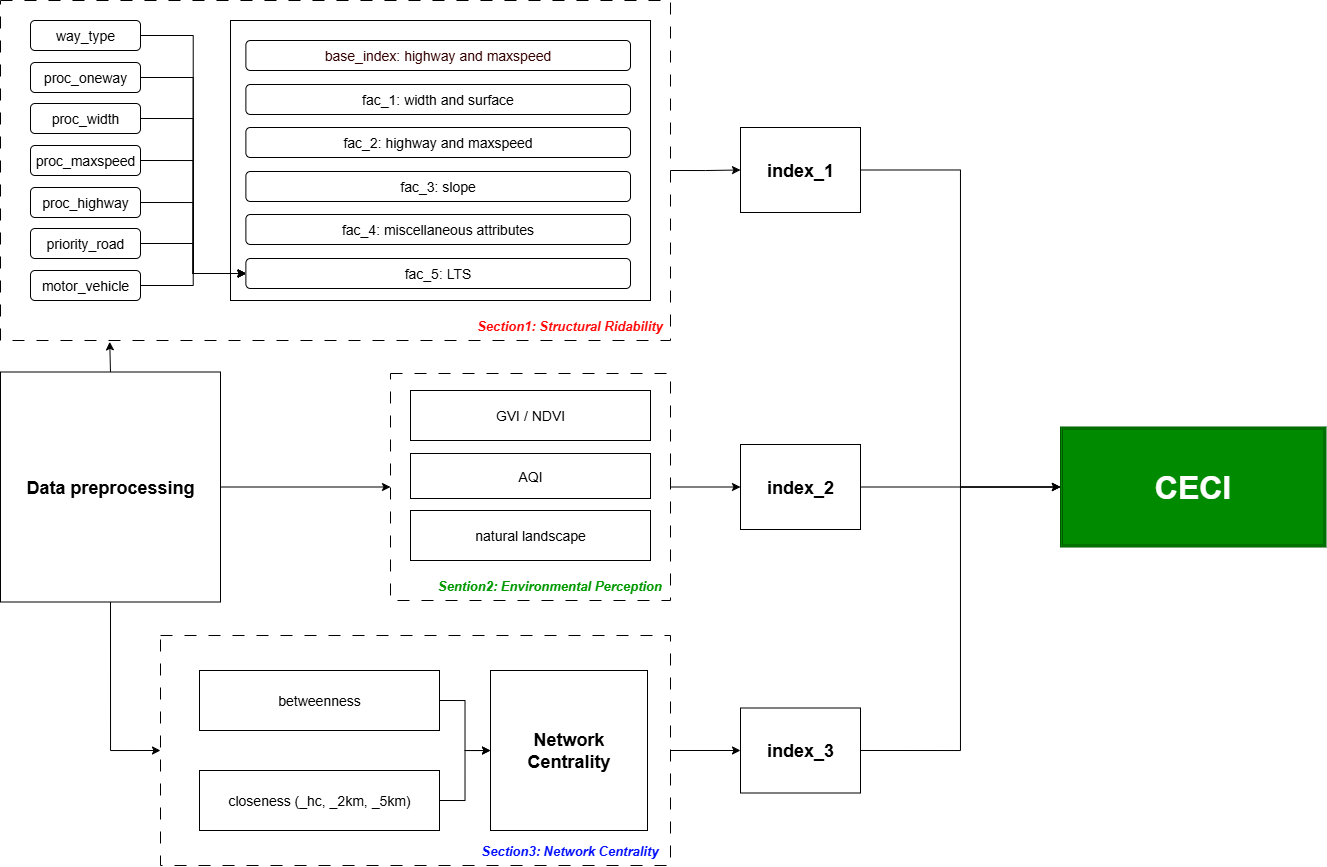
\includegraphics[width=1\linewidth]{general_images/flow} 

}

\caption{Workflow of the Composite Cycling Environment Index (CECI)}\label{fig:flow}
\end{figure}

Figure X summarises the end-to-end pipeline for constructing a link-level Composite Cycling Environment Index (CECI) for London. The workflow proceeds through four modules: (1) network acquisition and pre-processing, delivering a cleaned street graph and processed attributes; (2) a structural rideability module that assigns facility- and safety-related factors to each link and produces Index1; (3) an environmental perception module that aggregates greenery, air quality, and natural-landscape proximity into Index2; and (4) a network centrality module that computes graph-theoretic measures and yields Index3. The three sub-indices are winsorised and scaled to a common range and then combined into the CECI under a baseline equal-weights scheme, with predefined alternatives used for robustness. All operations are undertaken in EPSG:27700. Parameter values and rule tables appear in the Appendix to support reproducibility.

\section{Network acquisition and pre-processing}\label{network-acquisition-and-pre-processing}

\begin{enumerate}
\def\labelenumi{\arabic{enumi}.}
\tightlist
\item
  Extraction and selection
\end{enumerate}

The base street network is obtained from OpenStreetMap via a two-stage Overpass query. An inclusion-oriented stage captures bicycle-permissible ways across Greater London. A targeted clean removes motorways and ramps, under-construction segments, and links that explicitly prohibit cycling. Direction-dependent rules are implemented for left-hand traffic (\texttt{right\_hand\ traffic}=False).

\begin{enumerate}
\def\labelenumi{\arabic{enumi}.}
\setcounter{enumi}{1}
\tightlist
\item
  Topological and geometric cleaning
\end{enumerate}

A light-touch sequence improves graph consistency while preserving OSM geometry. Vertices within 2 m are snapped. Connected components with total length \textless{} 100 m are removed. Short dead-end stubs \textless{} 20 m are trimmed in three passes. Geometries are clipped to the Greater London boundary. Speed attributes recorded in miles per hour are converted to kilometres per hour (× 1.60934).

\begin{enumerate}
\def\labelenumi{\arabic{enumi}.}
\setcounter{enumi}{2}
\tightlist
\item
  Processed fields
\end{enumerate}

Pre-processing yields link-level attributes used downstream: \texttt{proc\_highway}, \texttt{proc\_maxspeed}, \texttt{proc\_width}, \texttt{proc\_oneway}, \texttt{priority\_road}, \texttt{motor\_vehicle}. These standardise tagging and encode London's traffic handedness.

\begin{enumerate}
\def\labelenumi{\arabic{enumi}.}
\setcounter{enumi}{3}
\tightlist
\item
  Normalisation convention
\end{enumerate}

Continuous metrics generated by later modules follow a common scheme: values are winsorised at the 1st and 99th percentiles, then min--max scaled to {[}0, 1{]}. Edge betweenness is transformed with log1p before scaling. Normalisation is applied within each sub-index prior to composite scoring.

\section{Structural rideability (Index1)}\label{structural-rideability-index1}

\subsection{Model Introduction}\label{model-introduction}

\begin{enumerate}
\def\labelenumi{\arabic{enumi}.}
\tightlist
\item
  Concept and provenance
\end{enumerate}

The structural module quantifies how road-segment design and operating conditions support everyday cycling. It draws on the open-source OSM Cycling Quality Index developed for Berlin (SupaplexOSM/OSM-Cycling-Quality-Index), which implements a deterministic, rule-based scoring system over OpenStreetMap data. In that reference model, link-level attributes parsed from OSM---such as functional road class and posted speed, cycleway tags (track/lane/opposite), number of lanes, separation and buffer treatments, surface/smoothness, parking configuration, and basic junction handling---are mapped through factor tables to penalties or bonuses. The Berlin implementation produces a link-level cycling quality score and a separate Level of Traffic Stress (LTS) classification using transparent, auditable rules derived from the above tags and thresholds. The intellectual lineage is acknowledged, and licence and repository details are provided in the Code Availability note.

\begin{enumerate}
\def\labelenumi{\arabic{enumi}.}
\setcounter{enumi}{1}
\tightlist
\item
  Adaptations
\end{enumerate}

The adaptation used in this research retains the central idea that compounding frictions are represented by multiplicative factors applied to a base score derived from functional class and speed, while re-specifying inputs and thresholds where necessary for the London context.

During model transfer, several source-model assumptions interact with country-specific OSM tagging practices and data completeness. In particular, the factor slot denoted as fac3 in the reference implementation collapses to a near-constant under London's OSM coverage (the driving attribute is sparsely or inconsistently recorded, yielding no informative variation at link level). To avoid carrying a non-informative term into the structural score, fac3 is re-specified as a terrain impedance factor derived from segment-level slope.

A further adaptation concerns the role of Level of Traffic Stress (LTS). In the reference framework, Level of Traffic Stress (LTS) and the Cycling Quality Index (CQI) are produced as parallel outputs. To determine whether LTS can be introduced as an additional structural factor within the composite (fac5 in Index1) without undue redundancy, a link-level multicollinearity check was conducted on the set \{LTS, fac1, fac2, fac4\}. Variables were standardised and analysed using principal components analysis (PCA); segments with incomplete structural attributes were excluded to ensure comparability.

PCA indicates a multi-dimensional structure rather than a single dominant latent factor. The explained-variance ratios are 43.31\% (PC1), 25.32\% (PC2), 17.18\% (PC3), and 14.19\% (PC4). Loadings show that LTS aligns chiefly with PC1, while fac4 overwhelmingly defines PC2; fac2 contributes strongly to PC1 and PC3, and fac1 loads on PC1 and PC4. The contrasted signs of LTS and fac2 on PC1, together with the near-orthogonal signal of fac4 on PC2, support the interpretation that these variables capture complementary dimensions rather than a single construct. Summary values are reported in Table X, and the geometry of loadings is visualised in Figure A (PCA biplot).

Variance inflation factors (VIF) provide a separate, regression-oriented perspective. LTS exhibits low collinearity (VIF = 2.03), with \texttt{base\_index} at a moderate level (= 4.63), while fac1 and fac2 show higher mutual dependence (= 27.73 and = 22.36). The low VIF for LTS combined with the PCA results indicates that LTS contributes additional information beyond fac1/fac2/fac4 and can therefore be retained as fac5 in Index1. The pairs plot and correlation matrix provided in the Appendix offer further diagnostic context.

Table X. PCA explained variance and loadings (absolute values).
(PC1 = 43.31\%, PC2 = 25.32\%, PC3 = 17.18\%, PC4 = 14.19\%)

\begin{table}
\centering
\caption{\label{tab:PCA}PCA table}
\centering
\begin{tabular}[t]{lllll}
\toprule
\textbf{Variable} & \textbf{PC1} & \textbf{PC2} & \textbf{PC3} & \textbf{PC4}\\
\midrule
stress\_level & 0.771 & 0.04 & 0.429 & 0.469\\
fac1 & 0.744 & 0.348 & 0.198 & 0.535\\
fac2 & 0.724 & 0.005 & 0.679 & 0.124\\
fac4 & 0.246 & 0.944 & 0.051 & 0.216\\
\bottomrule
\end{tabular}
\end{table}

\begin{figure}

{\centering 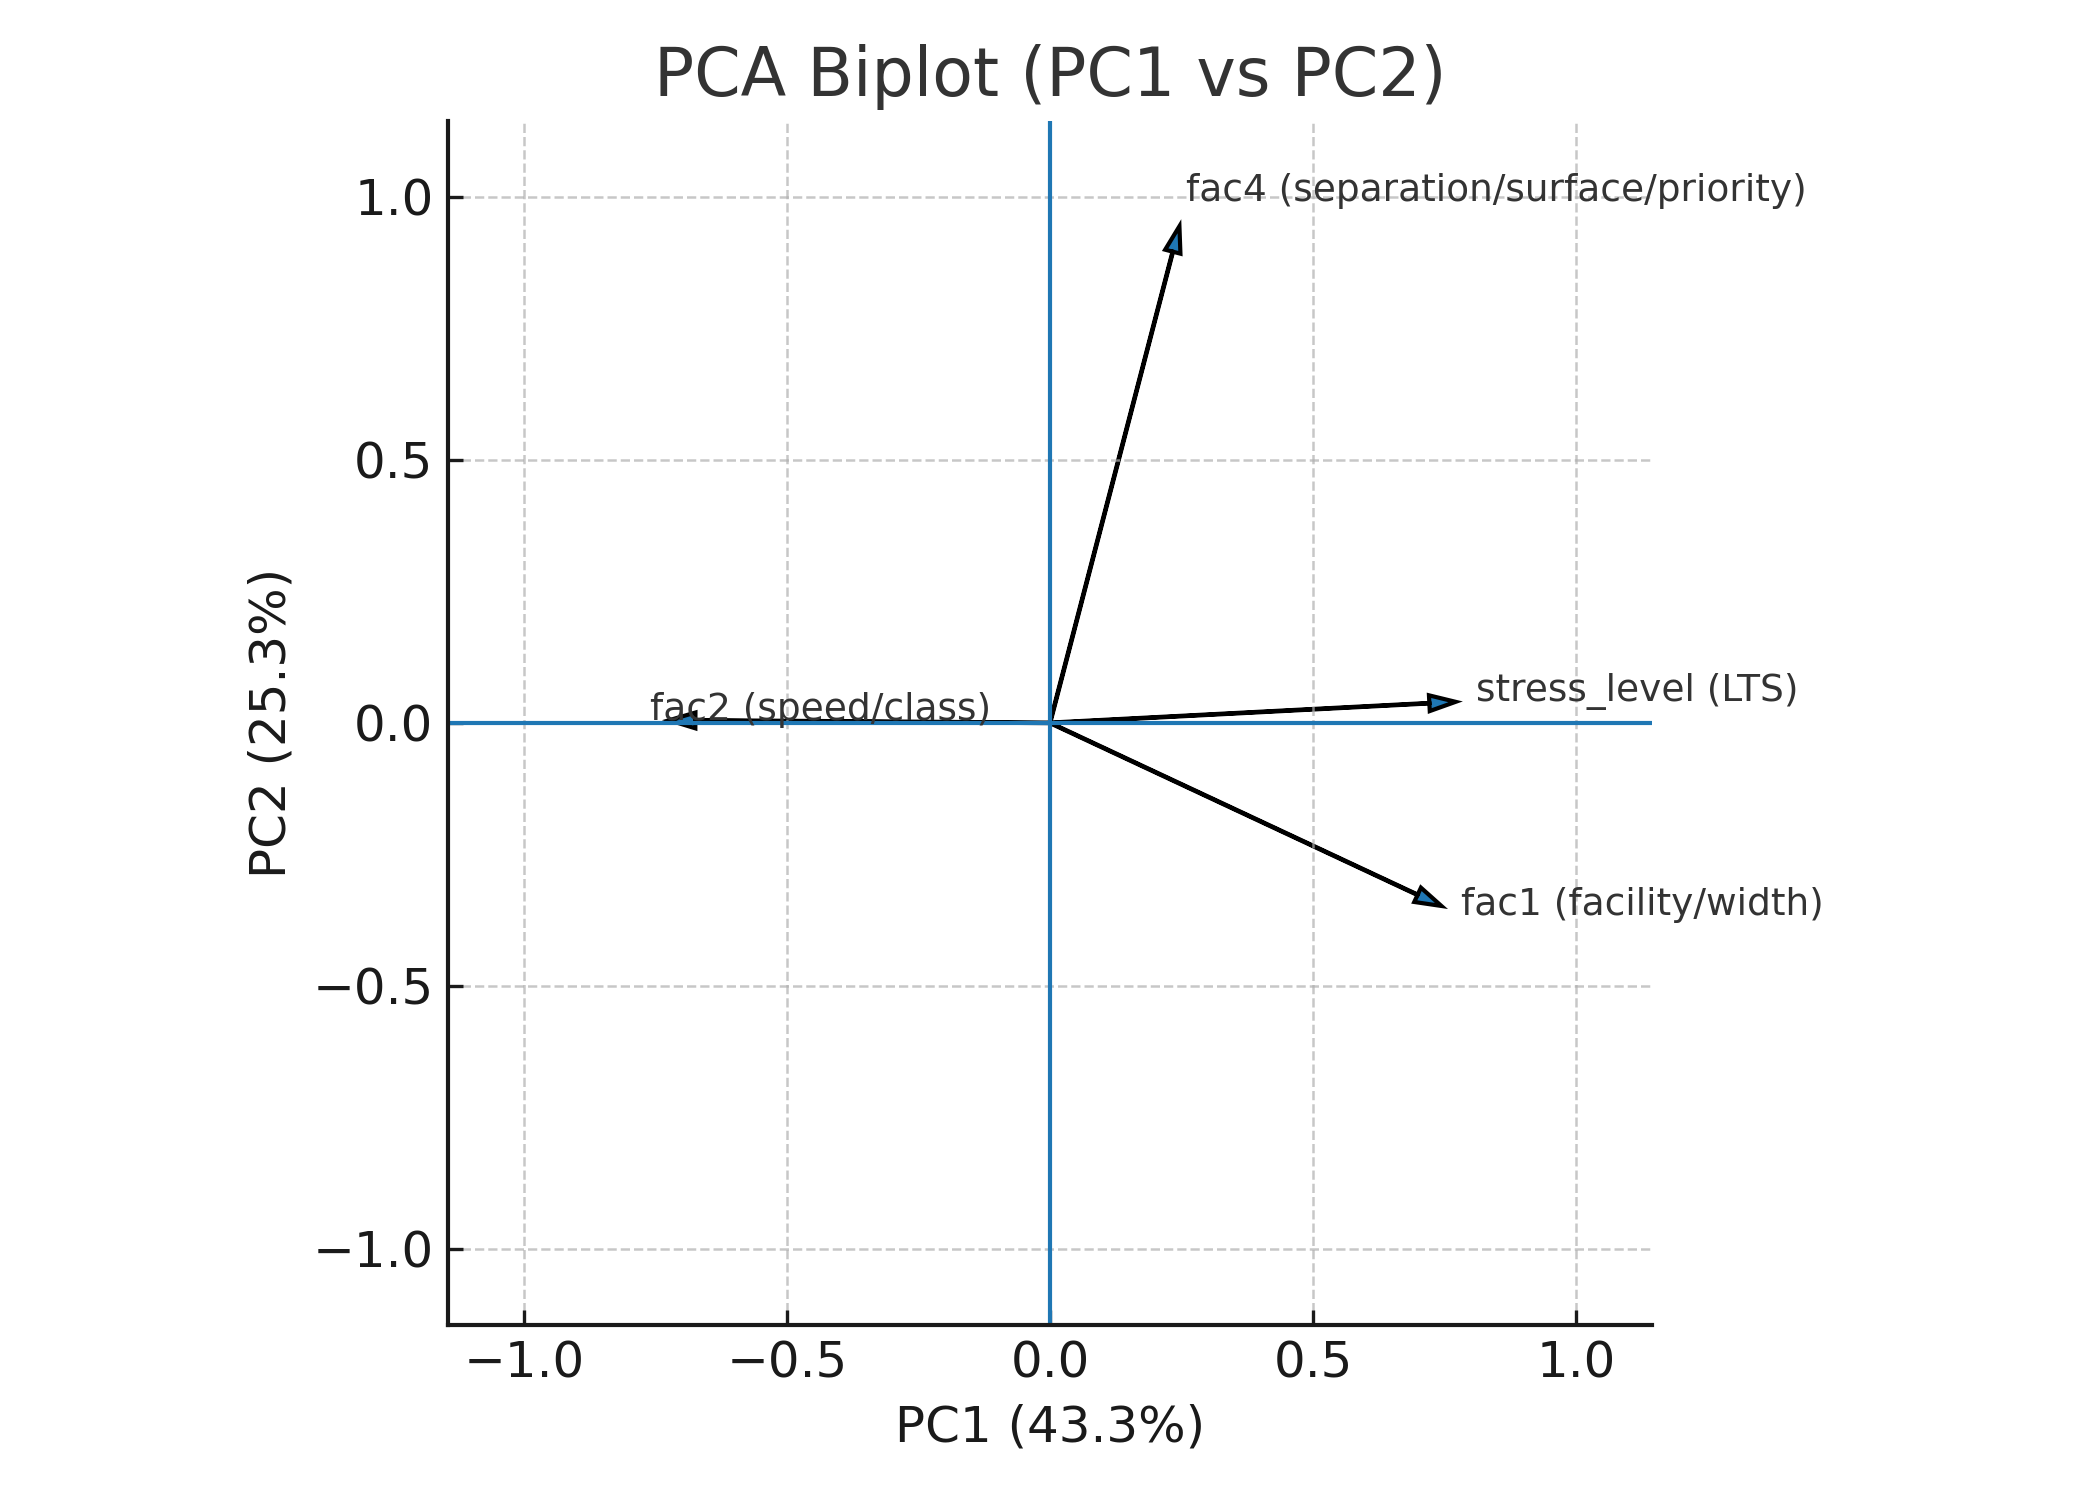
\includegraphics[width=0.9\linewidth]{general_images/pca} 

}

\caption{PCA biplot (PC1 vs PC2). Arrows denote variable loadings. LTS (stress level) aligns with PC1; fac4 defines PC2, indicating complementary dimensions.}\label{fig:pca}
\end{figure}

\begin{figure}

{\centering 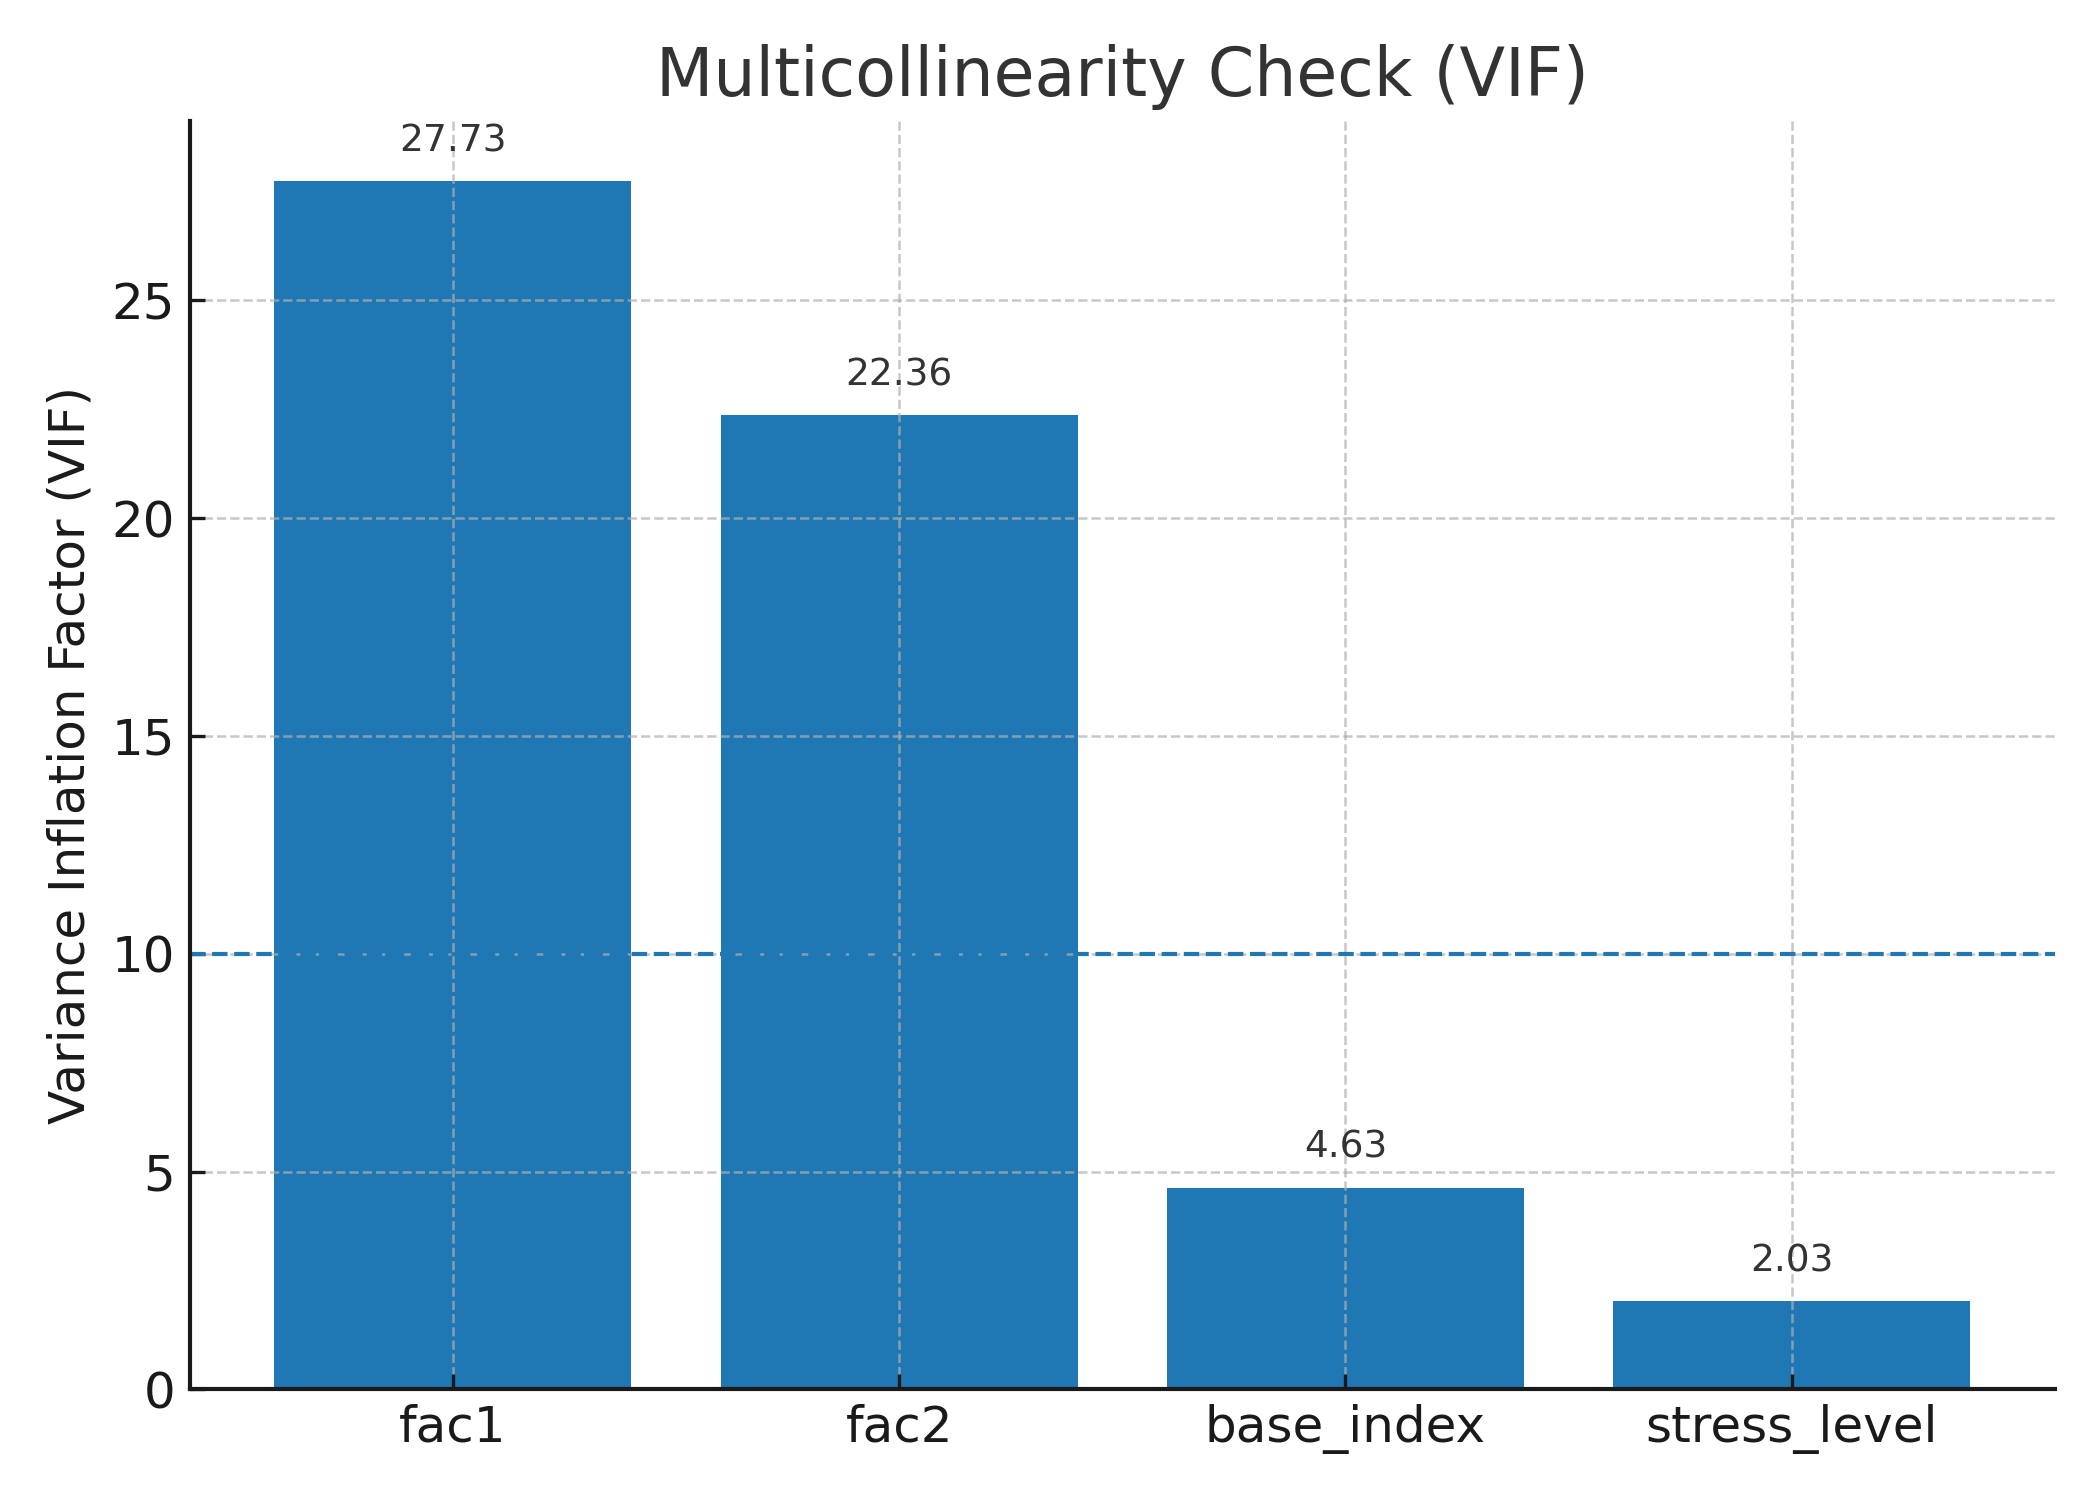
\includegraphics[width=0.75\linewidth]{general_images/vif1} 

}

\caption{Multicollinearity check (VIF). Bars show VIF for the structural variables used in diagnostics. LTS = 2.03, base index = 4.63, fac1 = 27.73, fac2 = 22.36.}\label{fig:vif1}
\end{figure}

These diagnostics justify retaining LTS as an independent factor in Index1, alongside facility/width (fac1), speed/class (fac2), and separation/surface/priority (fac4), within the multiplicative structural specification.

Also, there are some adaptations for left-hand-traffic regime, local speed patterns, and tag conventions to fit in with Great London.
The structural specification preserves the core Berlin logic while substituting a slope-based fac3 and justifiably incorporating LTS as fac5, yielding a London-tailored yet methodologically transparent module. Full parameter tables appear in the Appendix.

\subsection{Data preprocessing}\label{data-preprocessing}

A key element of preprocessing is sidepath identification. Because cycle facilities may be encoded on parallel geometries, a sidepath search prevents under-recognition of protection. Each main link is sampled every 100 m, and a 22 m search radius is used to detect cycle-designated paths. Where a sidepath is found, the main link inherits the relevant facility attributes for scoring, reflecting the facilities realistically available along the corridor.

\subsection{Engineered attributes and factor mapping}\label{engineered-attributes-and-factor-mapping}

Five categories of factors are computed from processed tags and terrain.

\begin{enumerate}
\def\labelenumi{\arabic{enumi}.}
\item
  Facility and width (fac1): Functional class together with cycleway:* tags and width inform a factor that rewards physically separated facilities and adequate operating width. Where width is unknown, conservative defaults are used (see Appendix). The mapping distinguishes protected tracks, painted lanes, advisory lanes, and mixed-traffic conditions.
\item
  Speed and classification (fac2): Posted speed (\texttt{proc\_maxspeed}) and \texttt{proc\_highway} class are combined to reflect exposure to motor traffic. Cut-points are calibrated to London's distribution of speeds and classes and are interpreted under left-hand traffic for oneway segments.
\item
  Slope (fac3): Terrain impedance is computed by sampling the 5 × 5 m slope raster along each geometry. Samples are aggregated to a representative segment value (robust statistic as specified in the Appendix) and then mapped to penalty factors. Missing slope receives fac3 = 0.9 as a conservative treatment that avoids unjustified improvement.
\item
  Separation, buffer, surface, and priority (fac4): Presence and width of buffers, type of kerb or median separation, parking configuration, surface/smoothness classes, and priority on major roads contribute additional penalties or bonuses. Directionality is evaluated with respect to left-hand traffic (e.g., parking or buffer on the rider's side). Rule tables provide deterministic mappings from tag combinations to factors.
\item
  Level of Traffic Stress (fac5): An LTS class is assigned from the joint configuration of speed, lanes, facility type, and separation (with junction handling consistent with local practice). Classes are translated into factors using the codebook values reported in the Appendix.
\end{enumerate}

\subsection{Base score and multiplicative formulation}\label{base-score-and-multiplicative-formulation}

A base score Base(highway, maxspeed) represents the nominal quality of a segment absent additional penalties or bonuses. The structural sub-index is:

\[Index_{1} = Base \times fac_{1} \times fac_{2} \times fac_{3} \times fac_{4} \times fac_{5}\]

followed by linear rescaling to {[}0, 100{]}. The multiplicative form ensures that simultaneously adverse attributes (e.g., steep gradient, high speed, lack of separation) reduce scores more than any single attribute alone, reflecting the compounding nature of perceived stress and safety constraints. Conversely, coherent design packages (e.g., protected track with buffer on a low-speed street) achieve proportionally high values.

\section{Environmental perception (Index2)}\label{environmental-perception-index2}

\subsection{Subcomponents and normalisation}\label{subcomponents-and-normalisation}

The environmental module operationalises three link-level components and combines them after normalisation.

\subsection{Greenery (GVI)}\label{greenery-gvi}

Link values are obtained by buffering each link midpoint by 30 m (or by regular along-link samples with the same radius) and averaging nearby GVI observations. Instances with no observations inside the buffer are recorded for transparency.

\subsection{Air quality (NO2)}\label{air-quality-no2}

The gridded NO2 surface (cell size 20 m) is sampled every 10 m along each link and averaged. The normalised value is inverted as (1 − \texttt{NO2\_norm}) so that higher values consistently denote better conditions.

\subsection{Natural-landscape proximity}\label{natural-landscape-proximity}

Polygons representing natural features are dissolved by type to avoid double counting. A multi-ring proximity function is computed around each link using the levels (50 m, 0.1), (40 m, 0.2), (30 m, 0.3), (20 m, 0.5), (10 m, 0.7), (1 m, 1.0); weights increase with proximity.

\subsection{Sub-index formulation}\label{sub-index-formulation}

After normalisation to {[}0, 1{]}, the three components are combined as:

\[Index_{2} = 0.5 \times GVI_{\text{norm}} + 0.3 \times (1 - NO_{2,\text{norm}}) + 0.2 \times Natural_{\text{norm}}\]

then rescaled to {[}0, 100{]}.

\section{Network centrality (Index3)}\label{network-centrality-index3}

\subsection{Graph representation}\label{graph-representation}

A primal, undirected graph is constructed from the cleaned OSM network. Edge weights equal metric length in metres.

\subsection{Betweenness}\label{betweenness}

Edge betweenness is estimated using approximate sampling with K = 1200 source pairs. Values are transformed with log1p and min--max scaled.

\subsection{Range-limited closeness}\label{range-limited-closeness}

Node closeness is computed within 2 km and 5 km network radii; edge-level closeness is the mean of endpoint values. A multi-scale composite is formed as:

\[C_{\text{multi}} = 0.6 \times C_{2\text{km}} + 0.4 \times C_{5\text{km}}\]

then scaled to {[}0, 1{]}.

\subsection{Sub-index formulation}\label{sub-index-formulation-1}

The centrality sub-index balances through-flow importance and local reachability:

\[Index_{3} = 0.4 \times Betweenness_{\text{norm}} + 0.6 \times C_{\text{multi,norm}}\]

rescaled to {[}0, 100{]}.

\section{Composite index, sensitivity, and reporting}\label{composite-index-sensitivity-and-reporting}

\subsection{Merging and keying}\label{merging-and-keying}

Outputs are joined by a stable key consisting of the OSM id and a hashed \texttt{edge\_uid} derived from endpoint coordinates. Geometry is inherited from the structural layer to maintain alignment.

\subsection{Composite scoring}\label{composite-scoring}

The composite index is the arithmetic mean of the three sub-indices under a baseline equal-weights assumption:

\[CECI = \frac{Index_{1} + Index_{2} + Index_{3}}{3}\]

This choice balances design quality, environmental comfort, and network position at evaluation stage. Length-weighted summaries may subsequently be produced for Borough or MSOA units for descriptive purposes; these aggregations are intentionally separated from model construction.

\subsection{Sensitivity analysis}\label{sensitivity-analysis}

To examine robustness to weighting assumptions, three alternative schemes are predefined:

\begin{itemize}
\item
  Scheme A (Index1/Index2/Index3): 0.5 / 0.25 / 0.25.
\item
  Scheme B (Index1/Index2/Index3): 0.25 / 0.5 / 0.25.
\item
  Scheme C (Index1/Index2/Index3): 0.25 / 0.25 / 0.5.
\end{itemize}

Comparative statistics and maps are reported alongside the baseline.

\subsection{Quality control and implementation notes}\label{quality-control-and-implementation-notes}

Post-cleaning checks review connectivity and degree distributions. Borough-level sidepath rates are monitored to flag tagging anomalies. Overlay steps (slope, greenery, pollution, natural features) record geometry--attribute counts to confirm coverage before index computation. Normalisation diagnostics document the effect of p1--p99 winsorisation. Processing uses standard Python geospatial libraries (GeoPandas, Shapely, rasterio, OSMnx) and graph tools with fixed random seeds. Parameter files and scripts are available in the project repository.

\chapter{Results}\label{results}

This section presents the empirical findings, beginning with an analysis of the components of structural ridability. It then assesses the environmental perception and network centrality. Finally, these dimensions are synthesized into a Composite Quality Index (CQI) to provide a holistic evaluation of London's cycling environment at multiple scales.

\section{Module 1: Structural Ridability}\label{module-1-structural-ridability}

The analysis of structural ridability reveals a two-layer constraint system governing cycling quality: the institutional status of a facility, captured by a base index, and its operational effectiveness, determined by secondary factors.

\subsection{Facility Type, Geometry, and Traffic Context}\label{facility-type-geometry-and-traffic-context}

\begin{figure}

{\centering 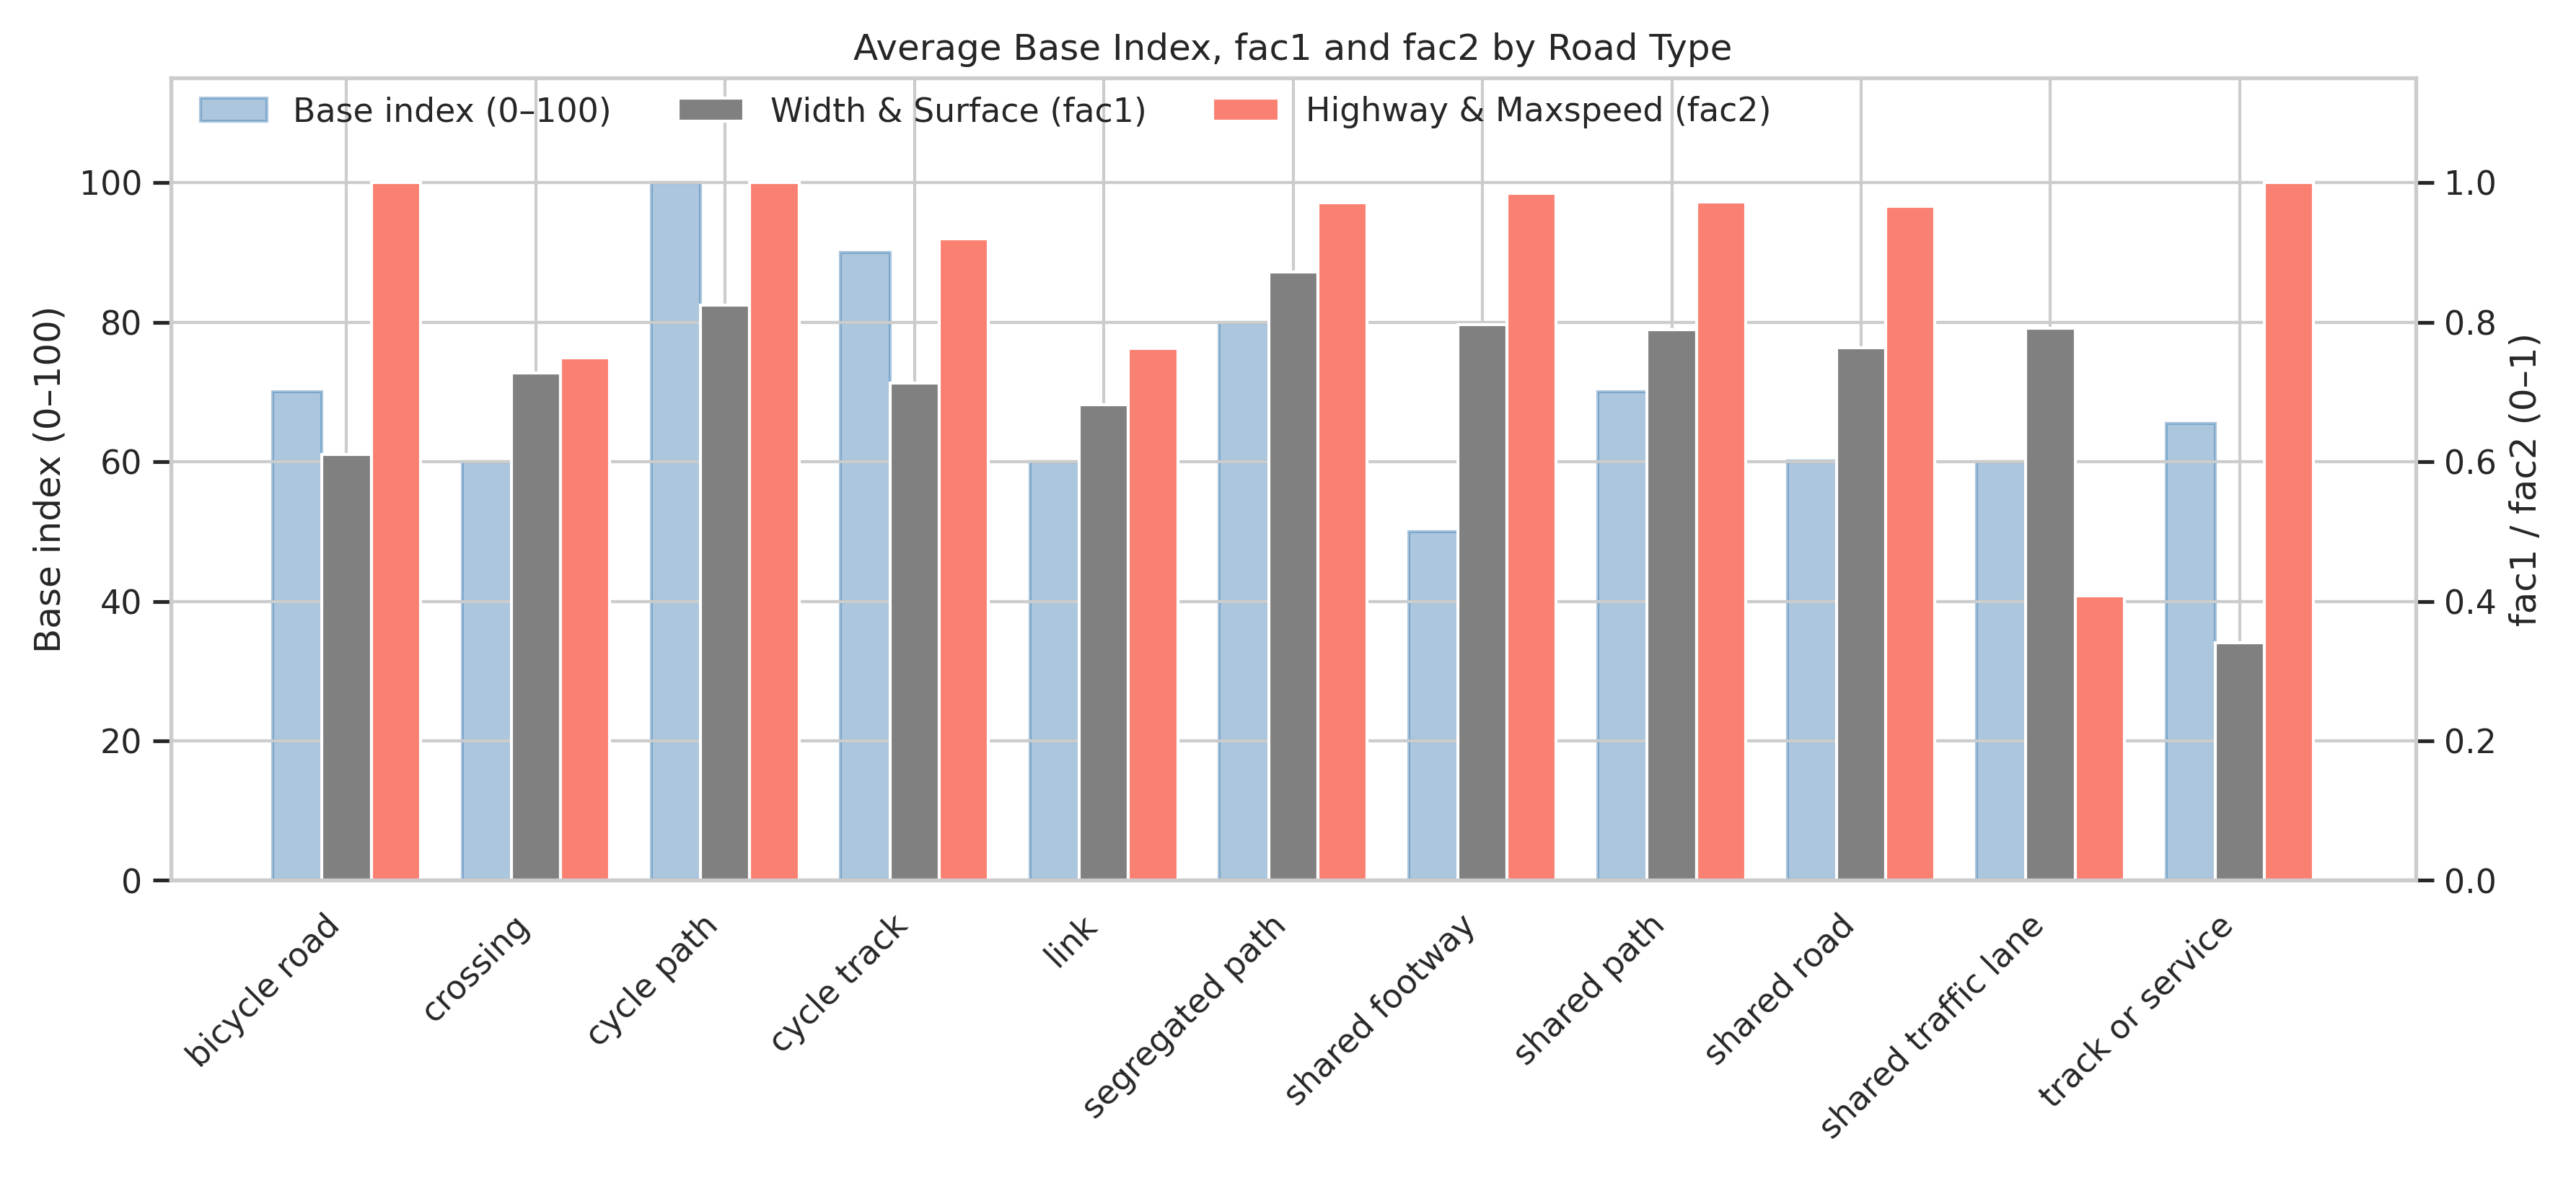
\includegraphics[width=0.95\linewidth]{general_images/fac1_2} 

}

\caption{Average Base Index, fac1 and fac2 by Road Type}\label{fig:fac12}
\end{figure}

The base index primarily reflects a facility's priority status. As shown in Figure X, dedicated infrastructure such as cycle paths (base index =100) and cycle tracks (=90) receive high baseline scores. In contrast, mixed-traffic or pedestrian-shared facilities, including shared footways (=50) and shared traffic lanes (=60), score substantially lower. This ``type prior'' rewards physical separation from motor traffic. This base score is then modified by two correction factors: fac₁ (width and surface) and fac₂ (road class and speed).

\begin{itemize}
\item
  Dedicated Facilities (Cycle Path/Segregated Path): These facilities exhibit high scores for both fac₁ (=0.78-0.88) and fac₂ (=1.0), indicating adequate width, good surfacing, and minimal adjacency to motor traffic.
\item
  Cycle Tracks: While fac₂ remains high (=0.9+), a slightly lower fac₁ (=0.70-0.75) suggests that localized geometric shortfalls, such as at bridge approaches or pinch points, can erode the advantage of a high base score.
\item
  Shared Roads: For shared roads, a low base score (=60) creates a ``type ceiling,'' capping the total index even with decent geometry (fac₁ = 0.76-0.80) and speed conditions (fac₂ = 0.95).
\item
  Shared Traffic Lanes: This category is constrained by a traffic bottleneck, evidenced by the lowest fac₂ score (=0.4) across all types. This indicates that mixing with motor traffic is the primary inhibitor of quality, regardless of geometry.
\item
  Track or Service Roads: These routes are constrained by geometry and surface quality, exhibiting the lowest fac₁ score (=0.34) despite having a fac₂ of approximately 1.0 due to low-speed environments.
\end{itemize}

\subsection{Topography and Traffic Stress}\label{topography-and-traffic-stress}

Beyond infrastructure, topography and traffic stress are key determinants of ridability.

\begin{figure}

{\centering \includegraphics[width=1\linewidth]{general_images/slopeLTS} 

}

\caption{Spatial distribution of slope (a) and Level of Traffic Stress (b) across Greater London.}\label{fig:slopeLTS}
\end{figure}

\begin{enumerate}
\def\labelenumi{\arabic{enumi}.}
\tightlist
\item
  Slope(\texttt{fac\_3})
\end{enumerate}

The spatial distribution of slope across Greater London reveals a distinct topographic gradient, with high-slope areas predominantly concentrated along the northern and southern peripheries of the region (Figure X). In particular, the southern belt exhibits continuous steep zones associated with the North Downs, while fragmented high-slope patches are observed in the northern uplands. By contrast, the central and eastern parts of London are characterized by extensive low-slope terrain, reflecting the dominance of the Thames floodplain and surrounding flatlands.

\begin{enumerate}
\def\labelenumi{\arabic{enumi}.}
\setcounter{enumi}{1}
\tightlist
\item
  LTS(\texttt{fac\_5})
\end{enumerate}

At the citywide scale, high-stress segments dominate the network. By link counts, LTS = 4 comprises 65.5\% (107,510 links) and LTS = 3 2.5\% (4,137 links), whereas low-stress LTS = 1 and LTS = 2 account for 18.6\% (30,444 links) and 13.4\% (21,985 links), respectively. This distribution indicates that, in its current form, London's cycling network primarily serves riders with greater experience or higher stress tolerance. Although low-stress facilities are widespread, they are largely fragmented and corridor-based, rather than forming a continuous citywide backbone.

Spatially, LTS = 1 ``blue corridors'' concentrate along motor-traffic-free or strongly separated alignments, including rivers/canals, greenways traversing large parks, and a subset of newly built or retrofitted segregated cycle tracks. These corridors are internally continuous, yet connections between corridors and into the metropolitan core are frequently severed by LTS = 3--4 segments. LTS = 2 is more common on lower-speed, lower-class residential streets, forming patches in the outer boroughs; however, inter-patch continuity is still constrained by LTS = 4 radial arterials and ring roads. LTS = 3--4 are widespread along primary/fast corridors, bridgeheads, and key connectors---locations that typically combine higher motor-traffic speeds and volumes or mixing with bus lanes---thus functioning as critical bottlenecks to network continuity.

These patterns are consistent with the classification logic: the script applies thresholding on way type, effective width, and speed limit, while also detecting sidepaths relative to adjacent motor carriageways. Facilities with physical separation or explicit cycle priority (cycle tracks/segregated/shared paths that satisfy width/speed criteria) are assigned to LTS = 1--2. Segments that mix with motor traffic, fall below width thresholds, or exceed 30 km/h speed limits are escalated to LTS = 3--4. In addition, shared/segregated paths that are not sidepaths are down-weighted for motor adjacency, biasing them toward lower LTS and producing the observed low-stress ``blue network'' along greenways, parks, and waterfronts. Where these routes must cross primary roads or bridges, the speed/width thresholds are triggered and stress increases sharply, yielding the red breakpoints observed in the map.

\subsection{\texorpdfstring{\texttt{Fac\_4}}{Fac\_4}}\label{fac_4}

Regression analysis shows that \texttt{fac\_4} contributes negligibly to the variation of \texttt{index\_1\_nor} (R² = 0.003). Although the coefficient is statistically significant (β = --26.91, p \textless{} 0.001), the explained variance remains below 1\%, confirming that \texttt{fac\_4} functions primarily as a correction factor rather than a substantive determinant of the index. Given its marginal explanatory power, \texttt{fac\_4} was not visualised separately in the results section but was instead acknowledged as an auxiliary adjustment within the index construction.

\subsection{Index of structural ridability}\label{index-of-structural-ridability}

\begin{figure}

{\centering \includegraphics[width=1\linewidth]{general_images/index_s1} 

}

\caption{Spatial Distribution of the Index of Structural Ridability}\label{fig:indexs1}
\end{figure}

The spatial distribution of the structural ridability index reveals a predominantly mid-range performance across London. As shown in the map and accompanying pie chart, nearly 70\% of road segments fall within the 15--25 and 25--35 bands, indicating that the majority of the cycling network provides only moderate levels of rideability. In contrast, low-value segments (0--15) remain limited, though not negligible, and are dispersed across multiple boroughs. High-value corridors (≥45) are comparatively rare but spatially clustered along specific arterial routes, suggesting that well-performing links tend to form isolated pockets rather than a continuous backbone. Overall, the results highlight a broad concentration around medium scores, with only a small proportion of routes delivering consistently safe and comfortable conditions.

\section{Module 2: Environmental Perception}\label{module-2-environmental-perception}

This module broadens the analysis to the perceptual and environmental context of cycling. A composite index was developed from three variables: Green View Index (GVI), NO₂ concentration, and natural landscape coverage.

\subsection{Green View Index (GVI)}\label{green-view-index-gvi}

\begin{figure}

{\centering \includegraphics[width=1\linewidth]{general_images/gvi} 

}

\caption{Hot and Cold Spot Analysis (Getis-Ord Gi*) of the Green View Index (GVI)}\label{fig:gvi}
\end{figure}

This is a GVI heat map, which shows that the distribution of people's perception of green landscapes is not random but exhibits a distinct clustering pattern. High-value clusters (hot spots) are predominantly located in areas with large urban parks, river corridors, and low-density residential neighborhoods, forming continuous belts of greenery. In contrast, low-value clusters (cold spots) are concentrated in the urban core, particularly around transport interchanges, high-density commercial centers, and major road intersections where vegetation is limited.

\subsection{NO₂ Concentration}\label{noux2082-concentration}

\begin{figure}

{\centering \includegraphics[width=1\linewidth]{general_images/no2} 

}

\caption{Spatial Distribution of Annual Mean NO₂ Concentration.}\label{fig:no2}
\end{figure}

The spatial distribution of NO₂ concentration mirrors the urban transport system. Elevated values are observed along major arterial roads, highways, and around transport hubs, forming a clear ``corridor effect.'' These areas, typically characterized by heavy traffic flow, exhibit persistent air quality challenges. By contrast, peripheral zones and green buffer areas display significantly lower concentrations, reflecting the mitigating effect of distance from vehicular emissions. The overall pattern highlights the dominant role of transportation emissions in shaping urban air pollution gradients, reinforcing the spatial inequality in environmental exposure across the study area (Figure X).

\subsection{Natural Landscape}\label{natural-landscape}

\begin{figure}

{\centering 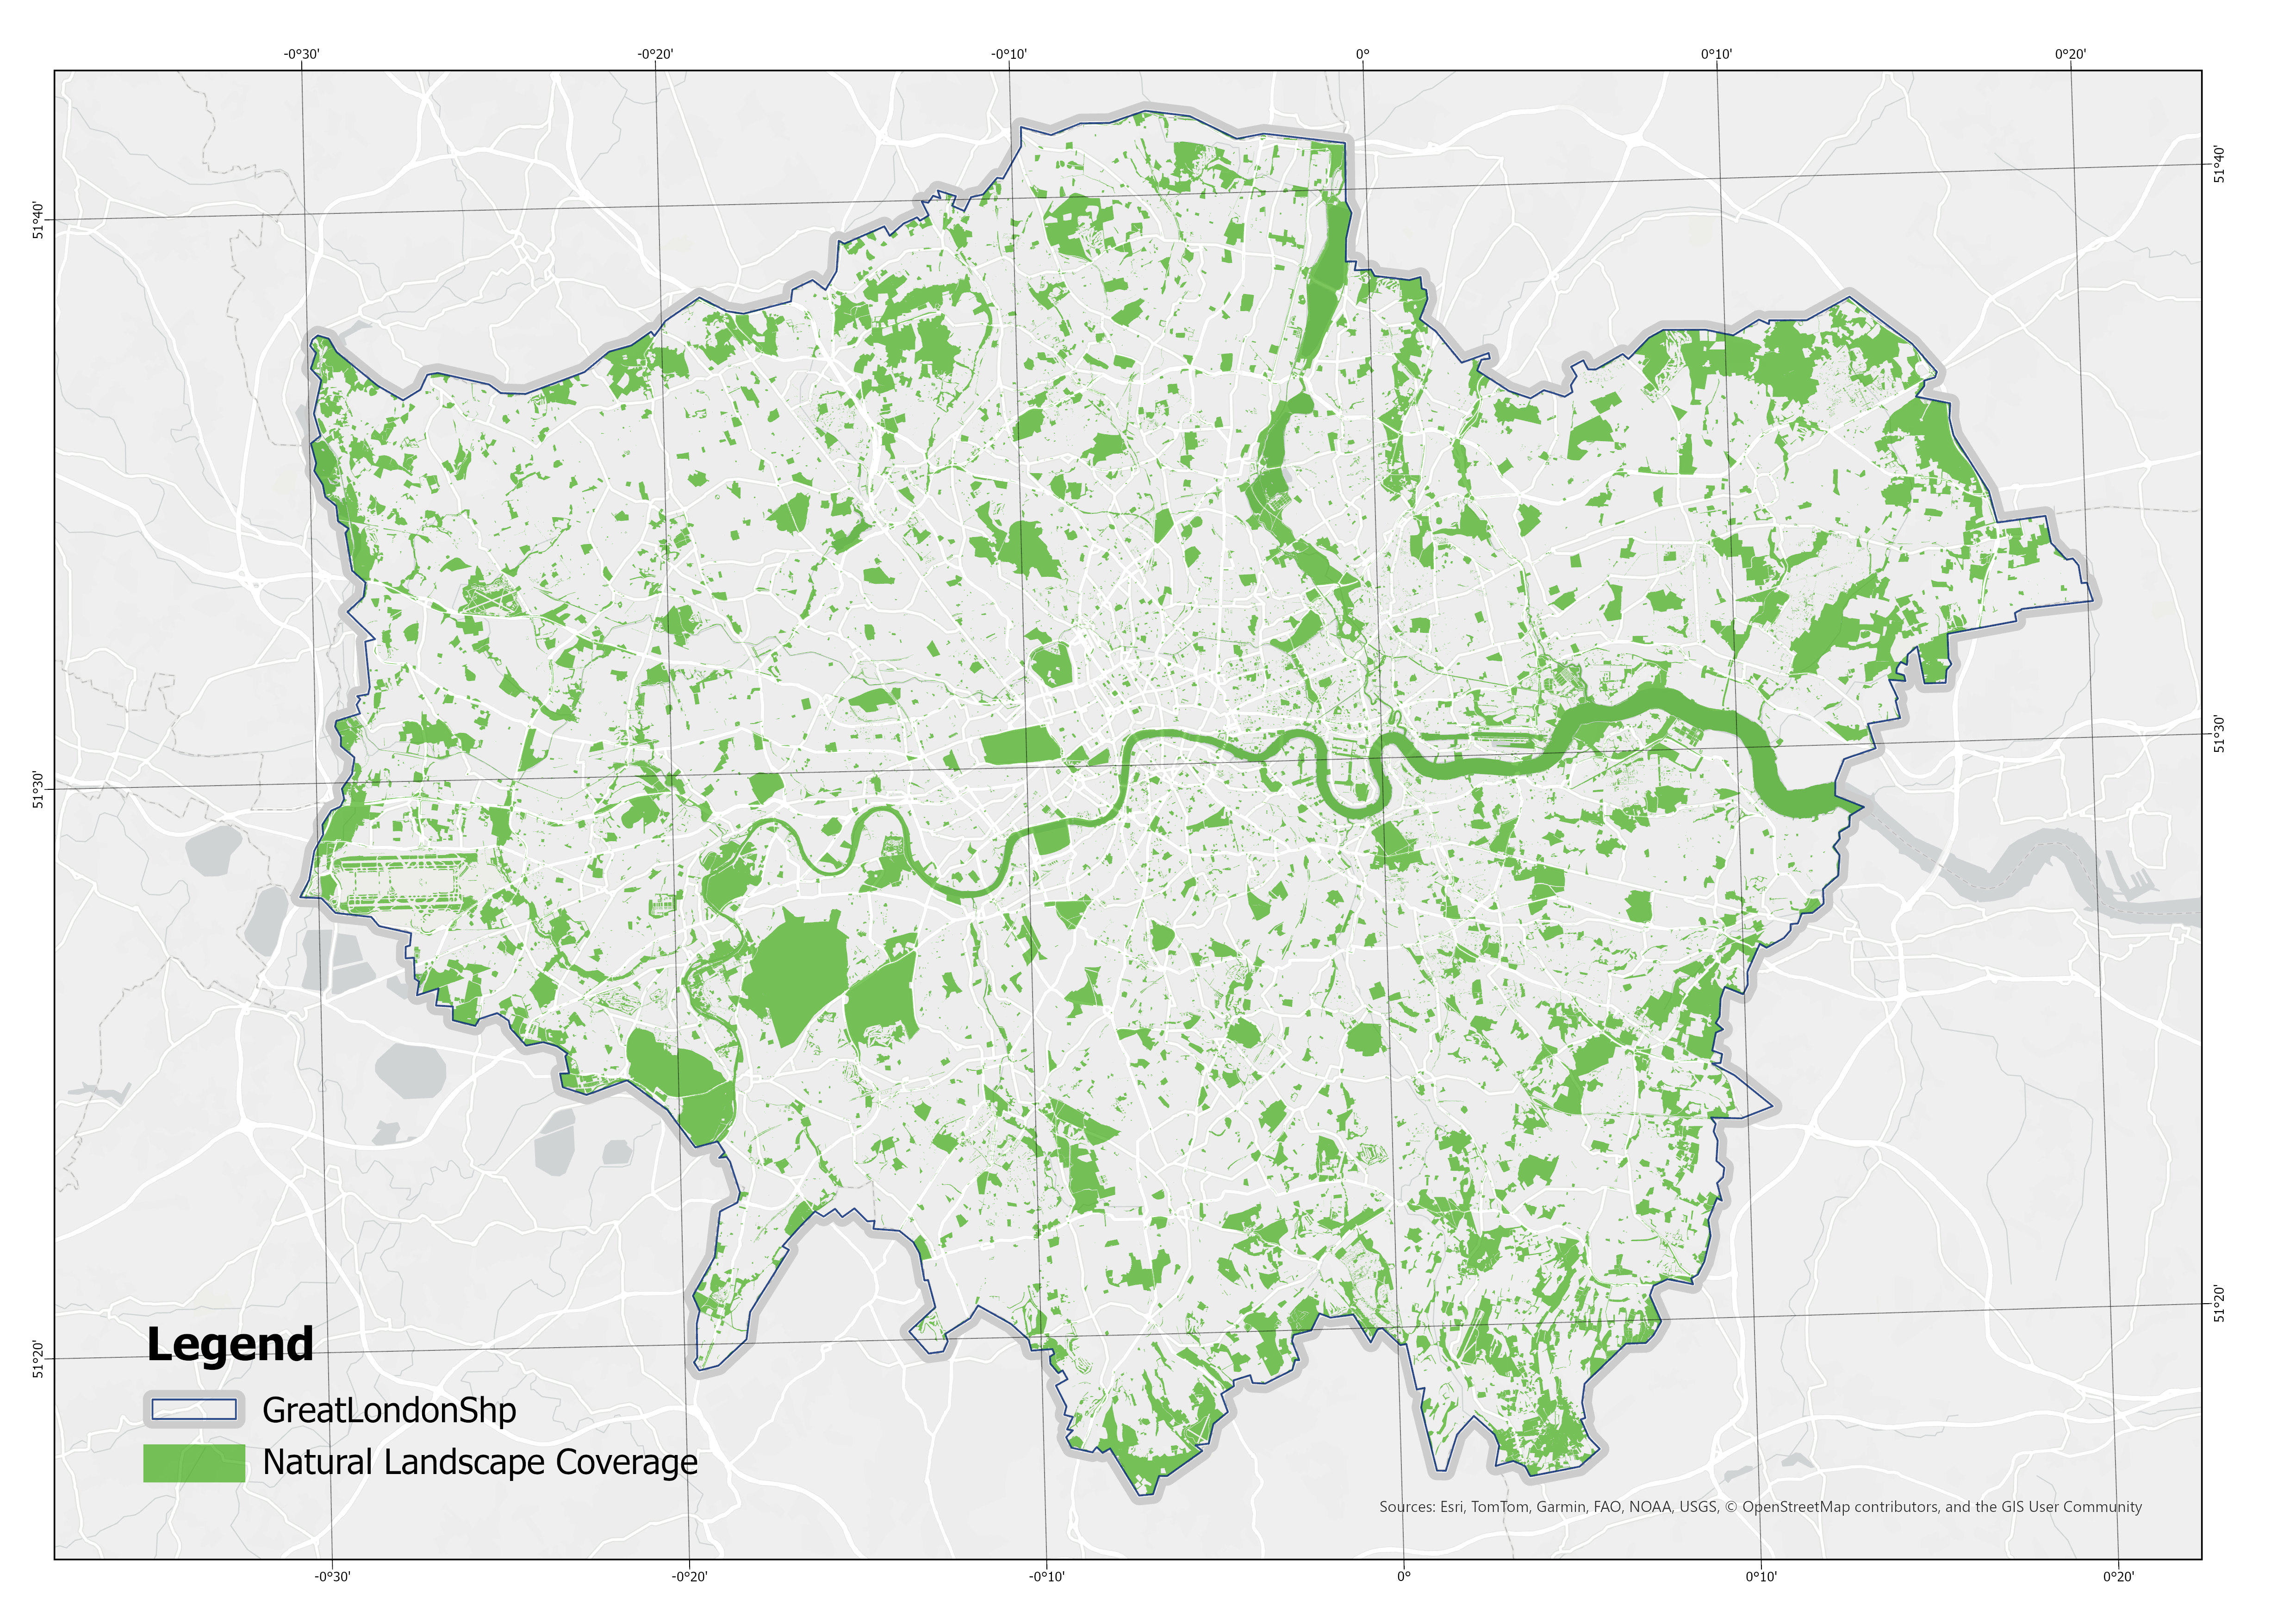
\includegraphics[width=1\linewidth]{general_images/nf} 

}

\caption{Spatial Distribution of Natural Landscape Coverage.}\label{fig:nf}
\end{figure}

The spatial distribution of natural landscape features presents a dispersed yet relatively balanced pattern. High-value clusters are concentrated along riverbanks, lakes, and peri-urban zones, forming ecological patches with visible continuity. In the urban core, the index values decline sharply, with natural landscape elements confined to isolated historical parks or large-scale public open spaces. This spatial pattern underscores the dominance of built-up land use in central districts while highlighting the ecological advantages of peripheral zones. The results suggest that natural landscapes in cities act as fragmented ecological enclaves that provide important, though unevenly distributed, ecosystem services (Figure X).

\subsection{Index of environmental perception}\label{index-of-environmental-perception}

\begin{figure}

{\centering \includegraphics[width=1\linewidth]{general_images/index_s2} 

}

\caption{Spatial Distribution of the Index of Environmental Perception}\label{fig:indexs2}
\end{figure}

When constructing the composite index that integrates GVI, NO₂, and natural landscape variables, a weighting adjustment was applied to account for the partial overlap between fac1 (GVI) and fac3 (natural landscape), both of which represent greenery-related attributes. Specifically, the weight of fac3 was slightly reduced to avoid redundancy. To ensure the robustness of factor integration, a multicollinearity test was conducted using correlation matrices (Figure X) and Variance Inflation Factor (VIF) statistics. The results confirmed that all variables have VIF values close to 1 (\texttt{fac\_gvi} = 1.077, \texttt{fac\_no2} = 1.039, \texttt{fac\_nat} = 1.057), indicating the absence of multicollinearity and supporting the rationality of the weighting scheme.

The resulting composite index demonstrates a distinct spatial gradient. High-value areas are primarily distributed in peripheral districts characterized by abundant green infrastructure and natural landscape patches, whereas low-value areas are concentrated in the city center, where limited greenery coincides with elevated pollution levels. This contrast highlights the compounded disadvantage faced by central urban districts, where deficits in environmental quality are most pronounced (Figure X).

In summary, the results from Module 2 reveal differentiated spatial patterns across three key dimensions of the urban environment---green visibility, air pollution, and natural landscape---and demonstrate the value of synthesizing them into a single composite indicator. The findings confirm that central urban areas consistently perform worse in terms of environmental livability, while peripheral districts benefit from greater ecological resources and lower pollution burdens. The multivariate analysis further validates that the integration of these factors is statistically robust and analytically meaningful. Collectively, this module provides a solid empirical foundation for evaluating urban environmental quality and supports the application of multi-factor composite indices in spatial planning and sustainability research.

\section{Module 3: Network Centrality}\label{module-3-network-centrality}

\subsection{Interpretation of Centrality Patterns in London's Road Network}\label{interpretation-of-centrality-patterns-in-londons-road-network}

\begin{figure}

{\centering \includegraphics[width=1\linewidth]{general_images/Centrality} 

}

\caption{Betweenness and Closeness Centrality in London's Road Network}\label{fig:Centrality}
\end{figure}

The spatial distribution of betweenness and closeness centrality in London's street network demonstrates a pattern that is consistent with the city's established urban structure. High values of both indices are concentrated in the central districts, particularly within the City of London, the West End, and adjacent areas along the Thames. This reflects the dense street configuration and the high level of interconnectivity, whereby these locations serve both as destinations of significant accessibility (closeness) and as critical intermediaries on shortest paths (betweenness).

Beyond the central core, radial arterials and major corridors exhibit elevated betweenness but comparatively lower closeness values. These road segments function as structural backbones of the metropolitan network, accommodating through-traffic and inter-district connections, but offering less balanced accessibility relative to the urban center. In contrast, peripheral suburban areas are characterized by low values of both measures, indicating their marginal role in the overall network in terms of both through-movement and spatial reachability.

The results also highlight the role of river crossings. Bridges along the Thames demonstrate disproportionately high betweenness centrality, reflecting their status as bottlenecks in the network that channel a substantial share of shortest-path flows across the river. This spatial concentration is consistent with the network dependency on limited crossing points.

\subsection{Index of network centrality}\label{index-of-network-centrality}

\begin{figure}

{\centering \includegraphics[width=1\linewidth]{general_images/index_s3} 

}

\caption{Spatial Distribution of the Index of Network Centrality.}\label{fig:indexs3}
\end{figure}

The composite centrality index demonstrates a highly uneven distribution across London's road network. High-centrality roads are concentrated within the central districts and along radial corridors, reflecting the city's monocentric structure combined with radial arterial organization. Peripheral suburban streets are predominantly located in the lowest centrality category, highlighting their marginal contribution to overall connectivity.

The proportional analysis further reveals that nearly 70\% of the road segments fall into the lowest category (\textless20), while only a small fraction of arterial and core streets attain values above 50. This imbalance underscores the hierarchical nature of London's road system, where a limited set of primary corridors sustains the majority of spatial accessibility and through-movement across the metropolitan area.

\section{Cycling Quality Index (CQI) Analysis}\label{cycling-quality-index-cqi-analysis}

Synthesizing the structural, environmental, and network metrics, the final Composite Quality Index (CQI) provides a holistic assessment of London's cycling environment.

\subsection{City-Wide Distribution and Bottleneck Identification}\label{city-wide-distribution-and-bottleneck-identification}

\begin{figure}

{\centering \includegraphics[width=1\linewidth]{general_images/cqi} 

}

\caption{Spatial Distribution of the Cycling Quality Index (CQI) by Quantile}\label{fig:cqi}
\end{figure}

The figure illustrates the Cycling Quality Index across Greater London, computed at the road-segment level and classified by quintiles. A pronounced core--periphery gradient is evident: low-value segments are densely concentrated in the inner city and central areas, while the outer boroughs gradually transition to medium and higher scores. Spatially, several continuous high-value corridors can be identified, most prominently along the Thames, canal routes, and selected upgraded arterials. However, these are frequently interrupted by low-value ``breakpoints'' at bridges, junctions, and complex intersections, reflecting the weakening of network continuity at critical nodes. In outer London, high-value links tend to appear as scattered patches, often connected to park greenways or local residential streets, but rarely forming coherent networks at a commuting scale.

Regionally, the most substantial cluster of low values is located within London's Central Activity Zone (CAZ), covering the Oxford Street--Strand corridor and its surrounding districts, including Soho, Covent Garden, and Bloomsbury. Here, the extremely dense street network, frequent intersections, and heavy motor traffic volumes contribute to persistently low index scores (0--35\% percentile), forming a continuous and extensive low-value core. This area not only constrains local cycling accessibility but also functions as a critical barrier, interrupting east--west and north--south connections between higher-quality corridors at the city-wide level.

In sum, London's cycling environment demonstrates a pattern of linear clustering along major corridors, widespread low-quality coverage on side streets, and insufficient continuity across rivers and key nodes. High-quality facilities are largely confined to linear routes and have not yet permeated the dense urban fabric.

\subsection{CQI Kernel Density Estimation in London}\label{cqi-kernel-density-estimation-in-london}

\begin{figure}

{\centering \includegraphics[width=1\linewidth]{general_images/cqi_kde} 

}

\caption{Kernel Density Estimation (KDE) of Low-CQI Road Segments}\label{fig:kde}
\end{figure}

This study applied kernel density estimation (KDE) to identify the spatial distribution of the Composite Quality Index (CQI). Road segments were sampled at 10 m intervals, CQI values were winsorised at the 1st--99th percentiles and normalised, and weighted points were aggregated on a 10 m grid with a 200 m Gaussian kernel. A separate surface was also generated for the top 20\% of CQI values to emphasise high-performing corridors.

The results show that clusters of low-CQI segments are predominantly concentrated in central and inner London, including the City and adjacent districts, where dense traffic flows and infrastructural pressure coincide with lower quality. Additional hotspots extend along several radial corridors, indicating stretches of consistently constrained accessibility and performance. In contrast, outer suburban areas exhibit weaker KDE intensity, reflecting fewer contiguous clusters of low-quality segments. These patterns highlight the uneven spatial distribution of deficiencies, with concentrations emerging in areas of high demand and structural significance.

\begin{itemize}
\tightlist
\item
  Stratford
\end{itemize}

A pronounced cluster of low CQI values is identified in the Stratford area of East London. This pattern is largely attributable to the hydrological configuration of the River Lea and its multiple distributaries, which fragment the street network and constrain lateral connectivity. As a result, movement is channelled through a limited set of arterial roads such as the A12 and Stratford High Street. While these main corridors demonstrate relatively higher quality, the surrounding secondary and local streets suffer from discontinuity and weak integration, which collectively depress the overall CQI in the area.

In contrast to the historic city centre---where a dense grid structure and abundant redundant links facilitate robust accessibility---Stratford's network is more vulnerable to fragmentation. The juxtaposition of a few strong arterial connectors with a wider set of poorly integrated local streets creates a marked cluster of low CQI intensity, underscoring the structural deficiencies induced by riverine segmentation.

\begin{itemize}
\tightlist
\item
  Isle of Dogs
\end{itemize}

The Isle of Dogs and its adjacent areas, including Rotherhithe to the west, North Greenwich to the east, and the northern edge around Limehouse, exhibit persistently low CQI values. This spatial pattern reveals significant structural deficiencies in the cycling network. Unlike motorised traffic, cyclists cannot rely on river tunnels such as the Blackwall Tunnel or the Limehouse Link, which officially prohibit or effectively restrict non-motorised access. The newly opened Silvertown Tunnel follows the same pattern, disallowing bicycles and offering only a limited shuttle bus alternative. As a result, cross-river cycling connectivity in this section of the Thames is severely constrained, and cyclists are forced into lengthy detours that substantially reduce network centrality.

Within the Isle of Dogs itself, the street system is dominated by inward-facing residential developments and cul-de-sacs, which further fragment the cycling network. While certain primary corridors maintain relatively higher scores, the absence of continuous east--west and north--south links suppresses overall accessibility. In contrast, central London benefits from a denser grid and multiple bridge crossings, providing cyclists with abundant routing options and higher network resilience. The combination of riverine barriers, restricted tunnel access, and local street discontinuities collectively explains the conspicuously low CQI in the Isle of Dogs region, highlighting the systemic limitations in cycling infrastructure integration across East London.

\begin{itemize}
\tightlist
\item
  Major parks
\end{itemize}

Several other large clusters of low CQI values are found within London's major parks. While such green spaces contribute positively to environmental perception, their functional characteristics inherently limit cycling network performance. In most cases, only a few primary corridors within or along the edges of the parks achieve relatively high CQI scores. However, the majority of internal routes provide limited infrastructure and weak network centrality, which substantially lowers the average quality within these areas. Given the extensive land coverage of these parks, these deficiencies aggregate into pronounced clusters in the KDE output.

\subsection{The CQI analysis at the borough level}\label{the-cqi-analysis-at-the-borough-level}

In order to conduct a more detailed analysis of the CQI in London, this study also carried out a graded analysis based on the borough as the scale.

\begin{figure}

{\centering 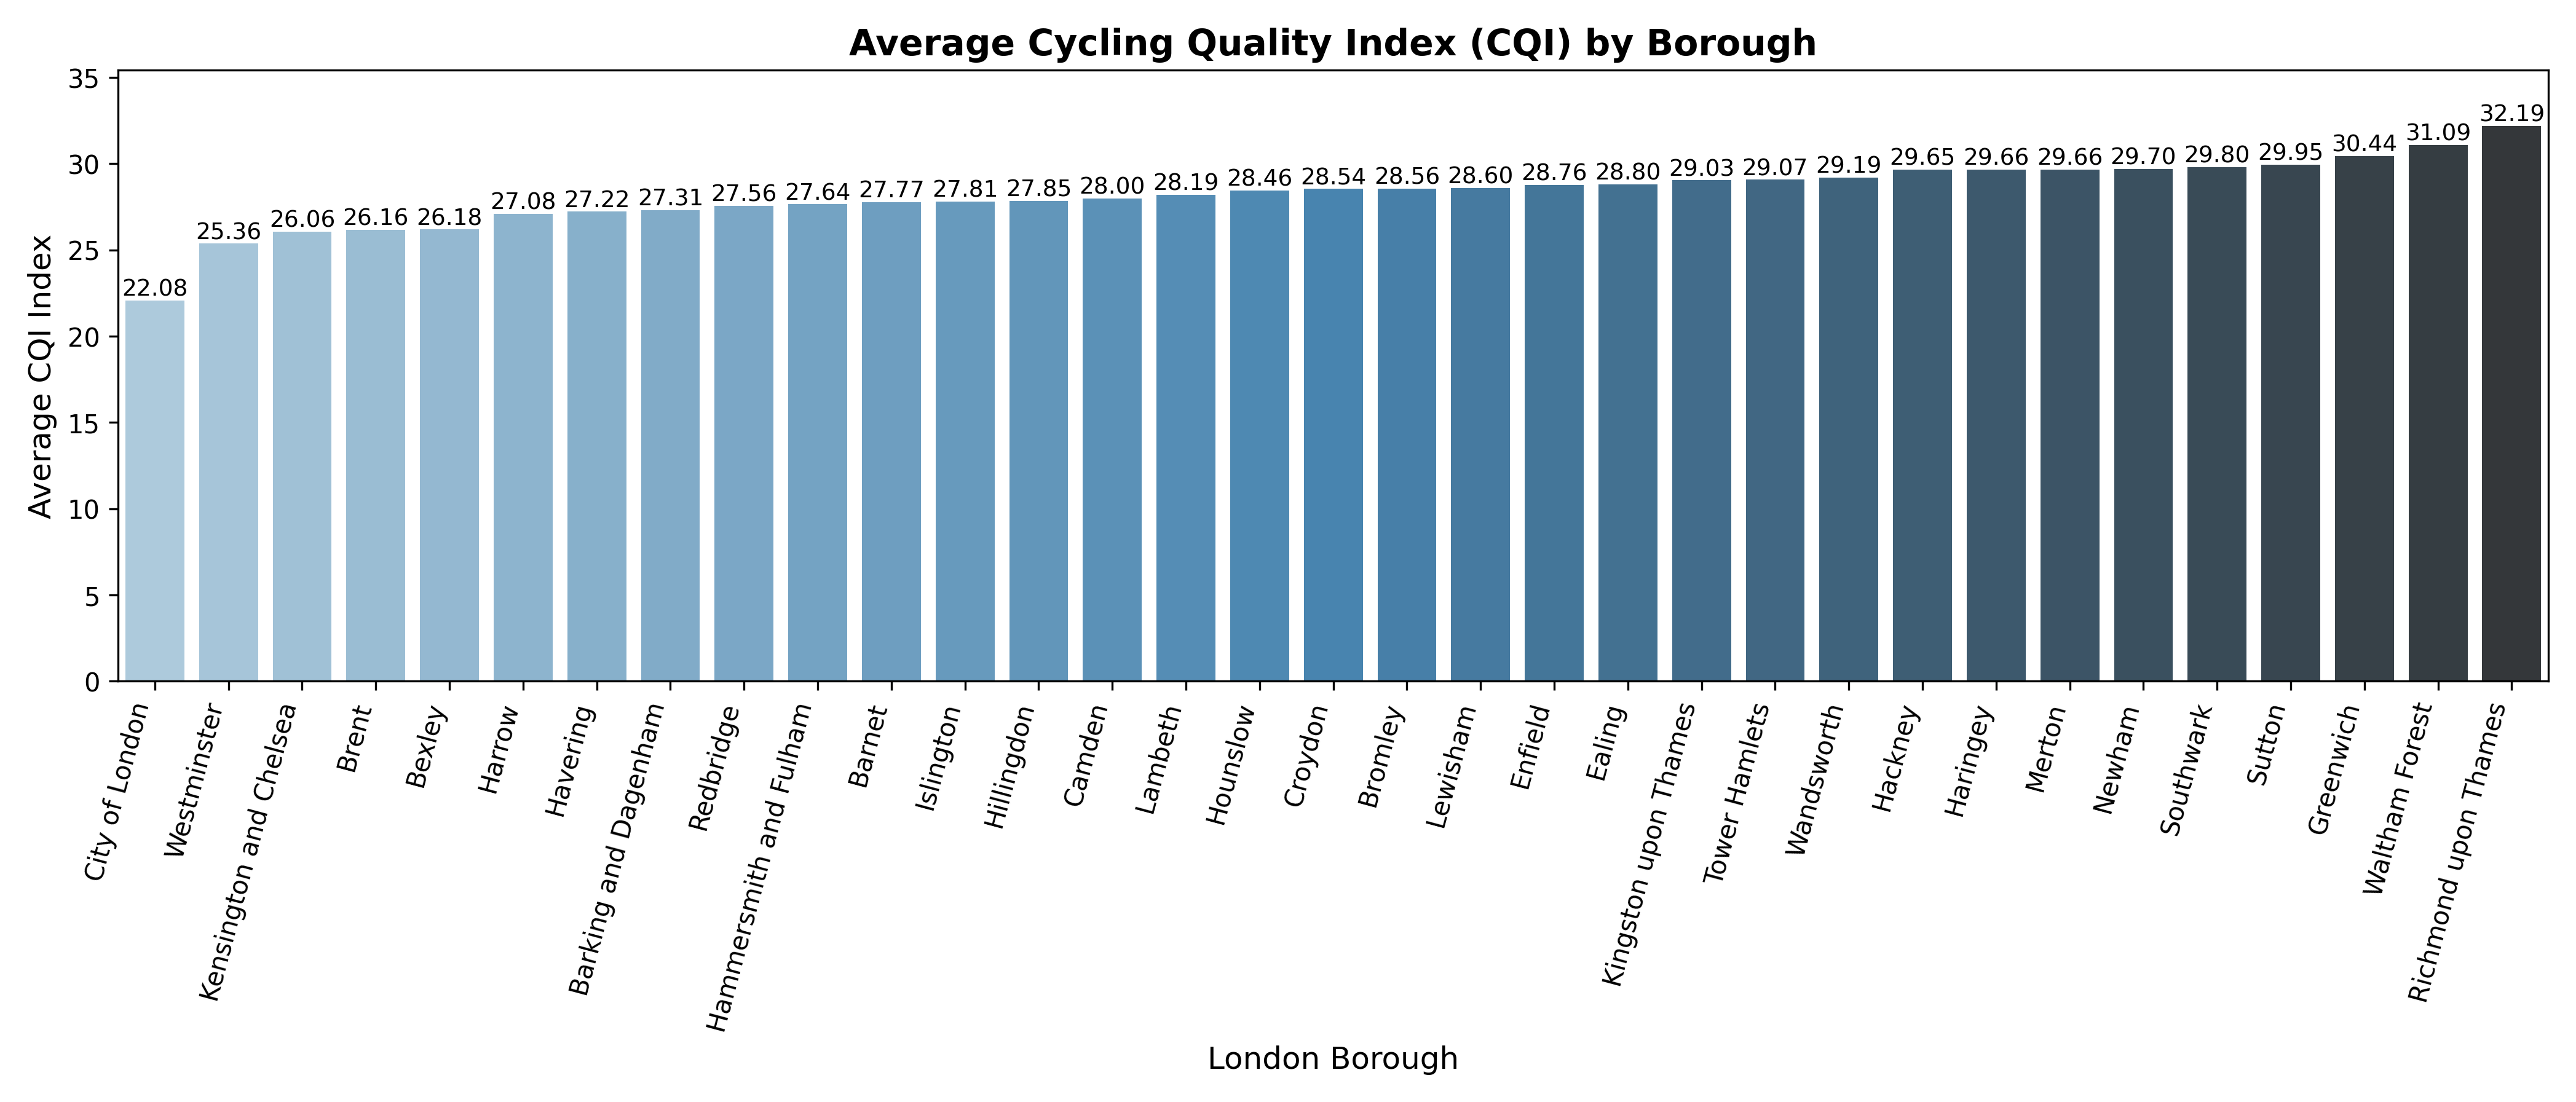
\includegraphics[width=1\linewidth]{general_images/AverageCQIbyBorough} 

}

\caption{Average Cycling Quality Index (CQI) by London Borough}\label{fig:AverageCQIbyBorough}
\end{figure}

By averaging the Cycling Quality Index (CQI) across boroughs, notable spatial disparities emerge. The highest-performing areas are Richmond upon Thames (32.19), Waltham Forest (31.09), Greenwich (30.44), Sutton (29.95), and Southwark (29.80), which all exceed the citywide mean and highlight relatively stronger cycling environments. In contrast, the lowest CQI values are observed in City of London (22.08), Westminster (25.36), Kensington and Chelsea (26.06), Brent (26.16), and Bexley (26.18), reflecting more constrained cycling conditions. This divergence suggests that central and inner boroughs with dense urban form and heavy traffic flows tend to perform worse, while outer or suburban boroughs with more space and dedicated infrastructure achieve higher quality levels. The results point to a spatial imbalance in cycling provision, where infrastructure quality does not align evenly with urban density and travel demand.

\begin{figure}

{\centering 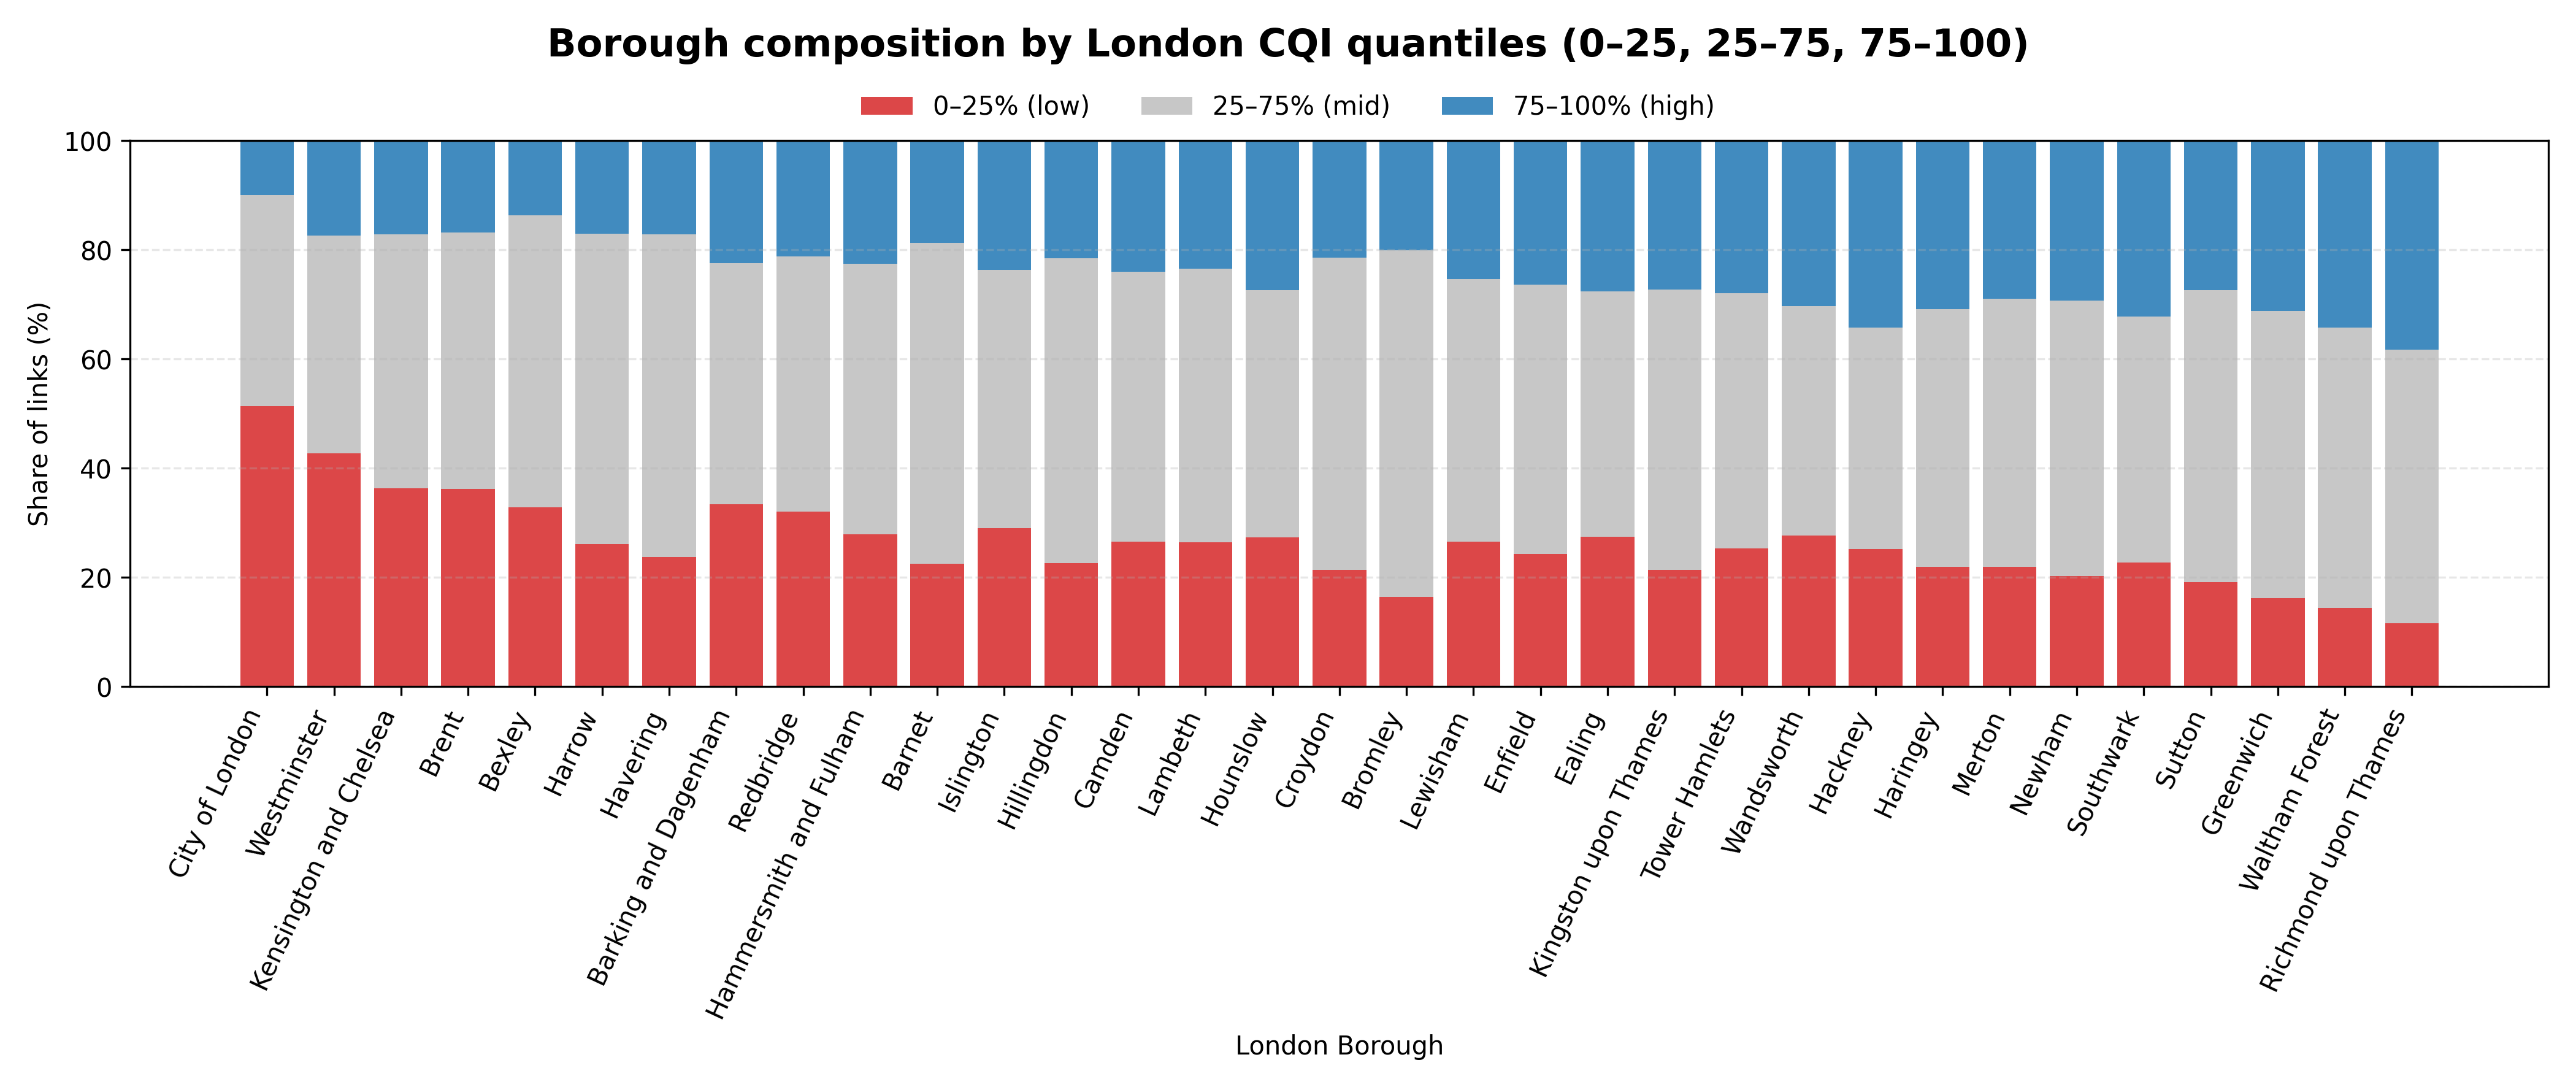
\includegraphics[width=1\linewidth]{general_images/BoroughComposition} 

}

\caption{Borough Road Composition by London-Wide CQI Quantiles}\label{fig:BoroughComposition}
\end{figure}

By examining borough-level road composition according to London-wide CQI quantiles, clear differences can be observed. The City of London shows the highest proportion of low-CQI links, highlighting its particularly constrained cycling conditions. For most boroughs, the share of mid-range CQI roads remains relatively stable, indicating that borough ranking is largely determined by the relative balance between high- and low-CQI segments rather than the middle category. This pattern suggests that differences in cycling quality across boroughs are more strongly driven by the extremes of infrastructure provision than by average conditions.

\begin{figure}

{\centering 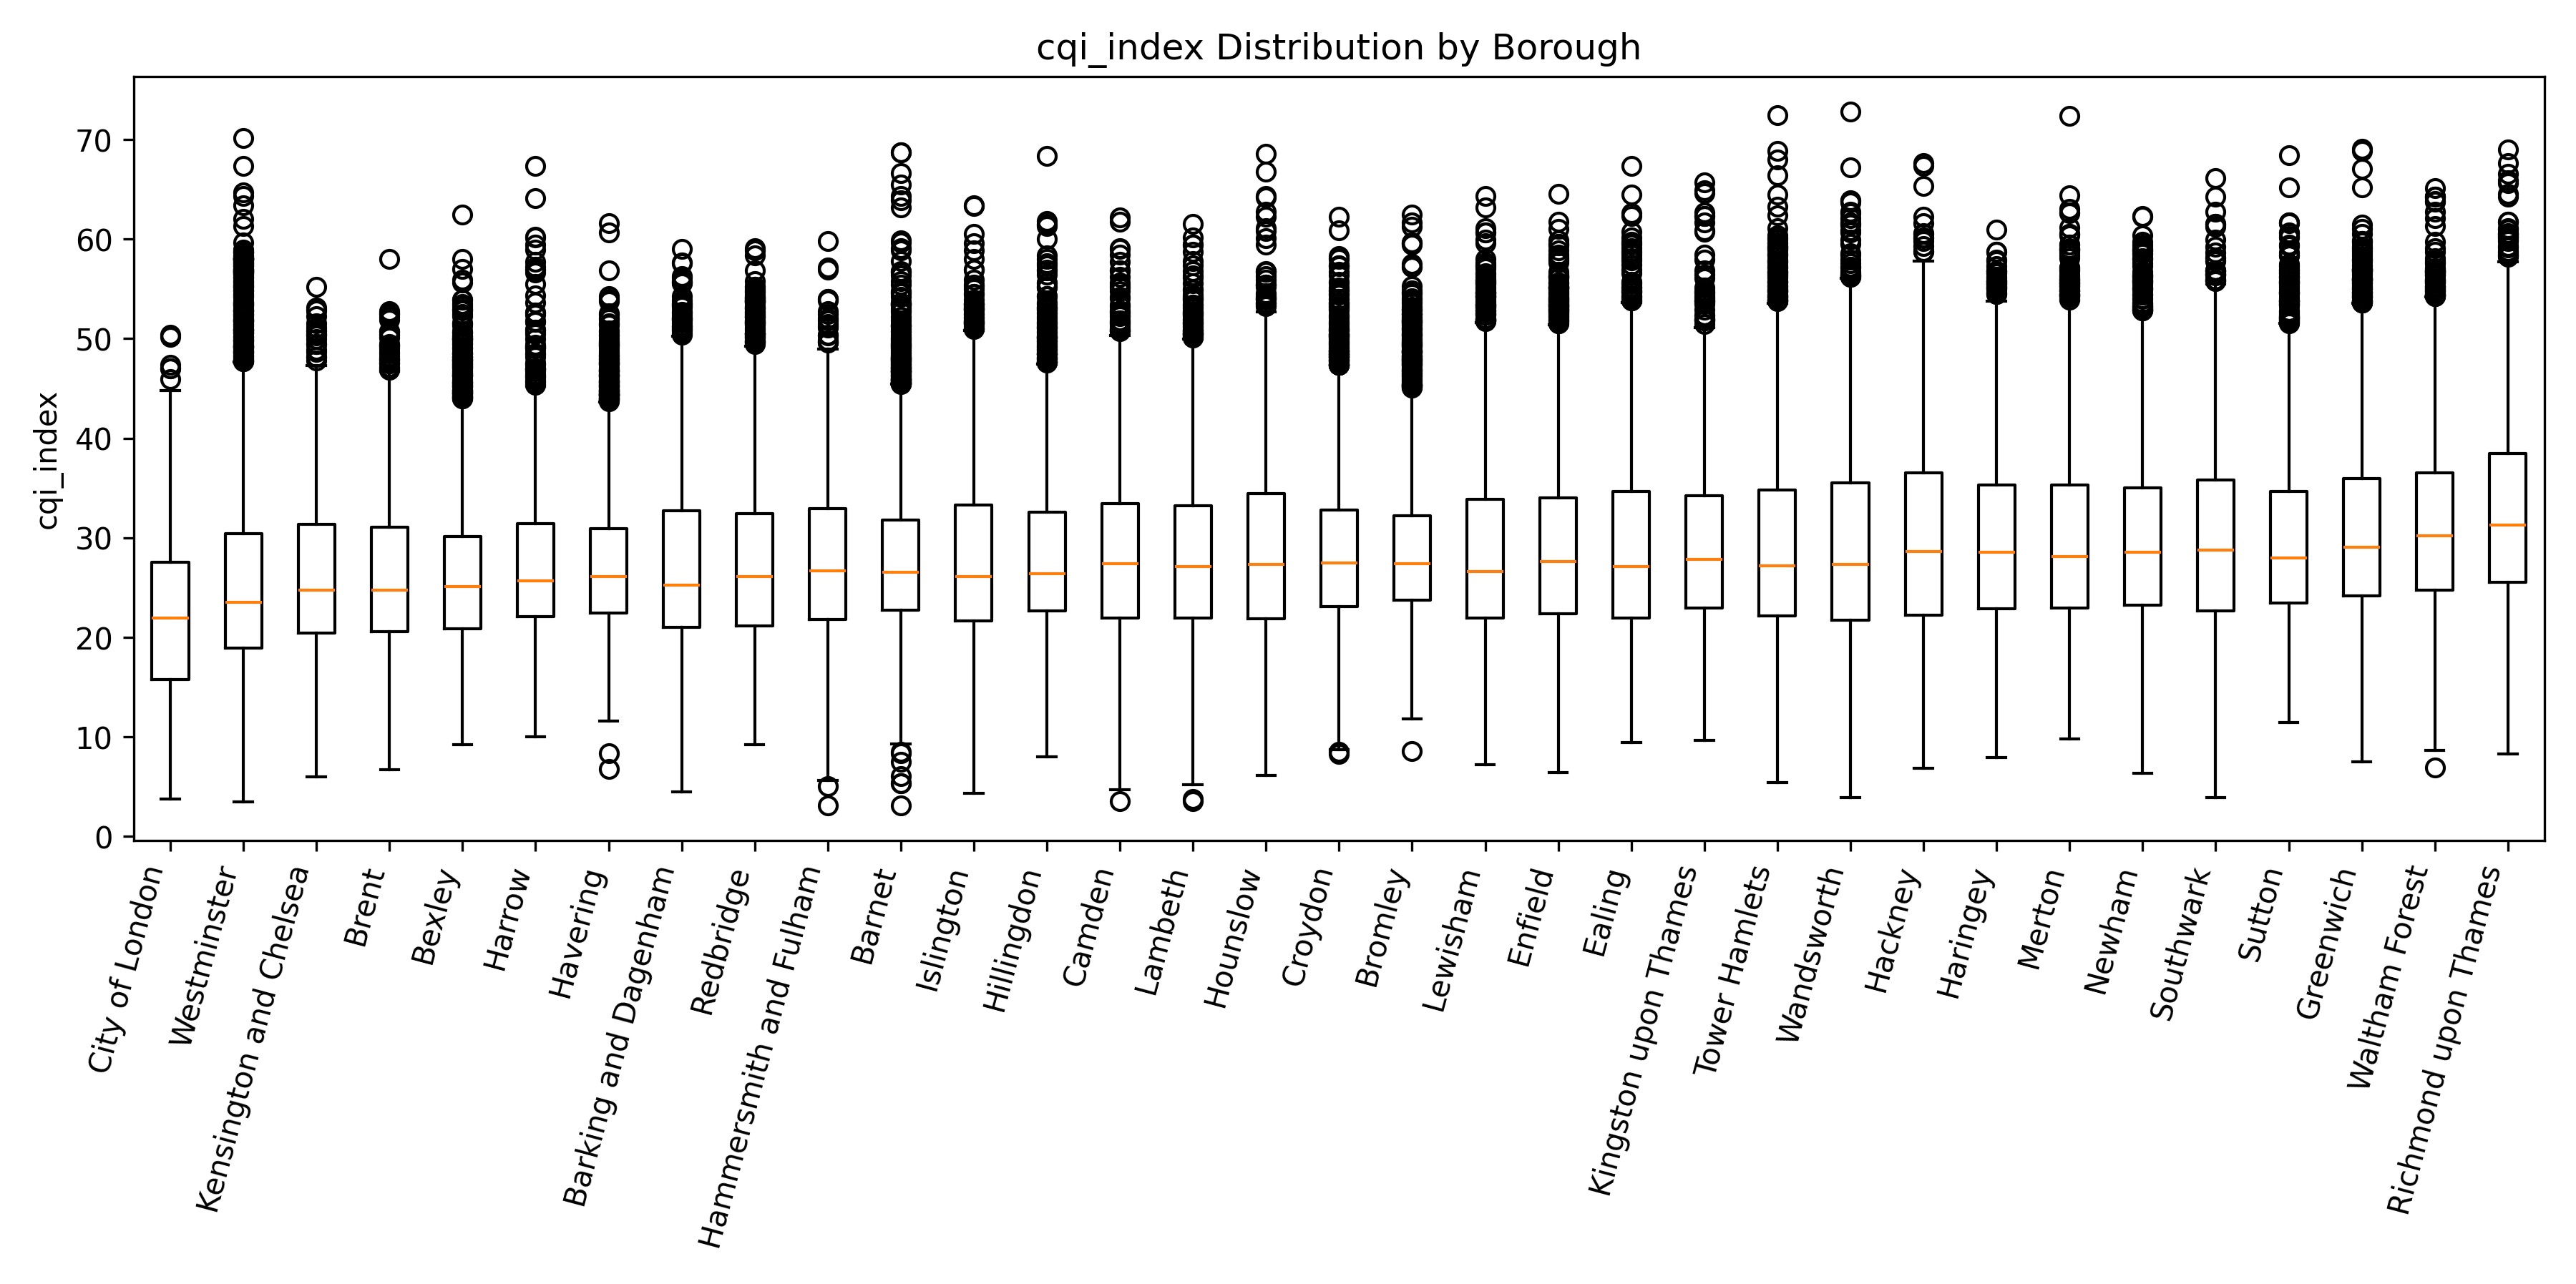
\includegraphics[width=1\linewidth]{general_images/box_cqi_by_borough} 

}

\caption{Distribution of CQI Scores within Each London Borough}\label{fig:boxcqiborough}
\end{figure}

To further examine intra-borough variation, Figure X presents the distribution of CQI scores for each borough. The results show that internal disparities are substantial across all boroughs. Even in the highest-ranked borough s, such as Richmond upon Thames and Waltham Forest, large interquartile ranges and overlapping distributions suggest that high cycling quality is not uniform but concentrated in selected corridors, while many other links remain only mid-performing. Similarly, in lower-ranked boroughs like the City of London and Westminster, the distributions are not only shifted towards lower medians but also highly dispersed, with numerous extreme low-CQI links. This highlights that borough-level averages can obscure significant within-borough inequalities: cycling environments are highly fragmented, and the experience of riders depends heavily on the specific routes available rather than the overall borough ranking.

\begin{figure}

{\centering 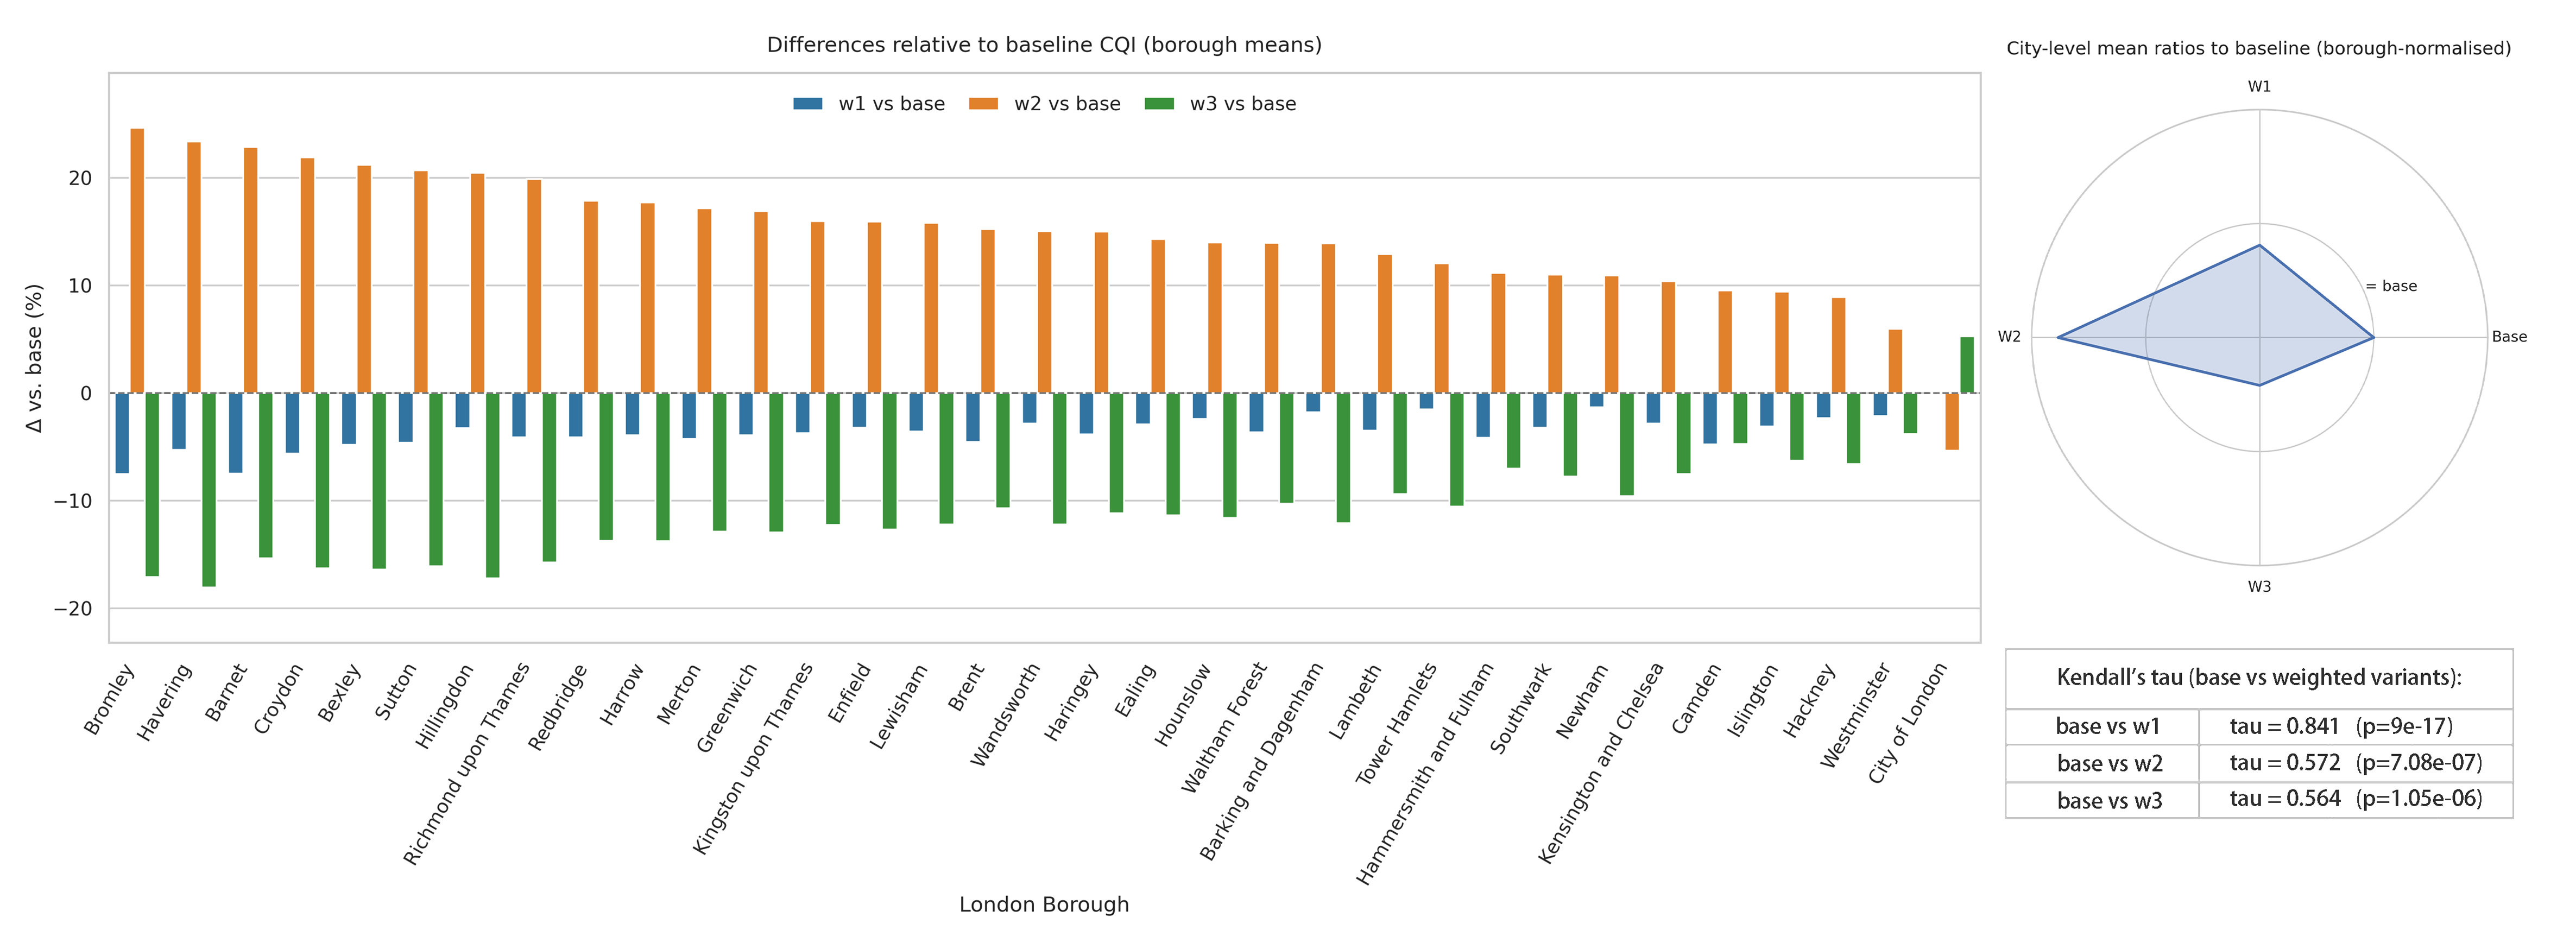
\includegraphics[width=1\linewidth]{general_images/cqi_robustness_delta_bar} 

}

\caption{Sensitivity Analysis of Borough Rankings under Alternative Weighting Schemes}\label{fig:cqirobustnessdeltabar}
\end{figure}

Sensitivity tests confirm that the equal-weight baseline is robust to moderate re-weighting. The alternative specification W1 shows negligible differences from the baseline (r=0.97, max \textbar Δ\textbar=7.5\%), indicating that small perturbations do not materially affect borough-level results. By contrast, prioritising Perceptual Environment (W2) raises overall CQI levels by approximately 10--25\%, whereas prioritising Network Centrality (W3) lowers levels by 8--18\%. These shifts are consistent with city-wide sub-index distributions, where environmental quality achieves relatively higher scores while centrality underperforms on average. Rank correlations further show that borough ordering remains broadly stable under W1 (τ=0.84) but undergoes moderate reconfigurations under W2 and W3 (τ=0.57). The low correlation between W2 and W3 highlights complementary spatial logics rather than redundancy. Therefore, the equal-weight index is retained for headline analysis, while W2 and W3 provide policy-relevant bounds reflecting amenity-oriented versus connectivity-oriented priorities.

\chapter{Discussion}\label{discussion}

Short introduction to the chapter, reviewing the previous chapter and detailing what this one aims to achieve and build upon.

\section{Research significance}\label{research-significance}

\subsection{Global development goals}\label{global-development-goals}

This study contributes to the wider agenda of sustainable development by addressing how active travel can be systematically evaluated and promoted. Cycling is explicitly connected to several United Nations Sustainable Development Goals (SDGs), including SDG 3 on good health and well-being, SDG 11 on sustainable cities and communities, and SDG 13 on climate action. By operationalising a composite measure of cycling quality, the research provides a framework for monitoring progress toward these goals. The findings highlight the need to improve accessibility, reduce exposure to environmental hazards, and ensure equity in mobility provision---key principles that resonate with international objectives for low-carbon, inclusive urban futures.

\subsection{Local policy}\label{local-policy}

At the local level, the dissertation provides evidence directly relevant to London's ongoing transport and environmental strategies. The identification of low-quality segments in the Central Activity Zone suggests that current investments in cycling infrastructure have yet to resolve issues of continuity and environmental stress in the city's busiest areas. The mapping of high-quality but disconnected corridors in outer boroughs also underscores the importance of linking peripheral areas to central employment hubs. These insights can inform initiatives such as the Mayor's Transport Strategy, the Healthy Streets Approach, and borough-level cycling action plans. By integrating infrastructural, environmental, and network perspectives, the CQI framework offers a tool for prioritising interventions where they can deliver the greatest impact.

\subsection{Academic research}\label{academic-research}

Academically, this study advances the growing field of urban cycling assessment by bridging methodological divides between infrastructure analysis, environmental perception, and spatial network science. While previous work has often focused on one dimension at a time, the composite index demonstrates the value of synthesising diverse indicators into a single evaluative framework. The approach responds to calls in the literature for multi-scalar, holistic assessments of urban mobility systems and contributes empirical evidence on London, a city that is often studied but rarely through an integrated, composite perspective. Beyond cycling research, the framework also illustrates how geospatial data, environmental metrics, and graph-theoretic measures can be combined in the analysis of urban accessibility.

\section{Limitations}\label{limitations}

The estimation of edge betweenness via stochastic source--target sampling imposes an inherent constraint on strict reproducibility. The sample size KK is chosen to balance run-time and stability, yet the procedure remains probabilistic; small numerical deviations and local rank shifts can arise across runs, and may be accentuated by differences in software versions, parallel execution order, or hardware. Under these conditions, the index is most appropriately interpreted through spatial patterns and relative ordering rather than exact equality of segment-level values across replications.

Temporal alignment across inputs constitutes a further limitation. The component datasets are not fully contemporaneous---street-level greenery is inferred from imagery circa 2015, modelled NO₂ fields originate from LAEI 2016 projections, and the OSM network is continuously updated. This asynchrony introduces the possibility of local timing mismatches, particularly where recent greening initiatives, traffic-calming schemes, or redesigns have occurred. As a result, fine-grained differences should not be read as current, time-specific conditions in all locations but rather as a structural and perceptual baseline.

Limitations also arise from cross-city parameter transfer within the structural rideability module. Thresholds and mappings for elements such as effective width, separation, and buffer rules derive from a framework calibrated in Berlin. Although the metadata in both contexts are sourced from OSM via Overpass Turbo, country-specific tagging practices, attribute completeness, and data conventions differ. During transfer, this heterogeneity can increase the frequency of missing or partially specified attributes. To avoid optimistic bias where attributes are absent, a conservative penalty mechanism is adopted that applies uniform downward adjustments under defined missingness conditions; this improves internal consistency but may produce a systematic downward shift in areas with sparser tagging.

The dependence on OSM further entails issues of coverage and tagging consistency. Volunteer-contributed data are uneven across space and over feature types, and fine-grained fields of particular relevance to cycling---cycleway subtype, buffer presence and width, surface and smoothness---may be omitted or inconsistently recorded. Such variation can propagate to factor assignment and to the stability of LTS classification, especially in neighbourhoods where infrastructure is evolving faster than tagging activity.

Design choices embedded in the network analysis also shape results. Centrality is computed on a primal, undirected, length-weighted graph, which abstracts from signal delay, turn costs, grade at junctions, and micro-routing preferences; the selected closeness radii and the approximate betweenness sampler represent defensible but not unique specifications. Similarly, distributional treatment through p1--p99 winsorisation and min--max scaling reduces the influence of extremes but compresses tail variation, with potential consequences for the relative prominence of isolated high- or low-scoring segments.

In addition, the composite weighting schemes encode normative assumptions regarding the relative salience of structural quality, environmental comfort, and network position. Alternative analytical or policy perspectives might reasonably prioritise these dimensions differently, yielding variation in spatial rankings. Taken together, these considerations indicate that the index should be interpreted as a comparative, spatial diagnostic rather than as a definitive, time-specific measure of present conditions.

\section{Transferability}\label{transferability}

A further significance of this research lies in its transferability to other urban contexts. The CQI framework is built on widely available datasets and reproducible geospatial methods, making it adaptable to cities beyond London. While local calibration would be necessary to reflect different infrastructural standards, environmental conditions, or policy priorities, the general approach of integrating structural rideability, environmental perception, and network centrality is applicable to diverse settings. This opens avenues for cross-city comparisons and benchmarking, enabling researchers and policymakers to assess cycling environments in a consistent way. By doing so, the framework supports broader efforts to mainstream active travel within sustainable mobility agendas globally.

\chapter{Conclusion}\label{conclusion-1}

This dissertation has developed and applied a composite framework for evaluating the cycling environment of London, addressing the interplay between infrastructural conditions, environmental perception, and network connectivity. The research was motivated by the need to move beyond fragmented assessments of cycling quality and to deliver a holistic tool that can highlight disparities and guide targeted interventions. Through the construction of a Cycling Quality Index (CQI), the study has provided new insights into the spatial distribution of cycling opportunities and constraints across Greater London.

The findings revealed a marked core--periphery gradient, with central districts characterised by high traffic stress, fragmented facilities, and environmental burdens, while outer areas contained more isolated but higher-quality segments often associated with parks and green corridors. Importantly, the analysis showed that no single dimension is sufficient for evaluating cycling quality: infrastructural improvements may be undermined by environmental pressures, while attractive green routes may fail to deliver connectivity. By integrating these factors into a unified index, the study contributes both methodologically, by operationalising a replicable evaluation tool, and empirically, by providing one of the most detailed portraits of London's cycling environment to date.

\section{Recommendations}\label{recommendations}

Based on the findings, several recommendations are offered:

\begin{enumerate}
\def\labelenumi{\arabic{enumi}.}
\item
  Strengthen central network continuity
  Investments should prioritise filling infrastructural gaps and reducing bottlenecks in central London, where demand is highest but network fragmentation and environmental stress are most acute. Upgrading crossings, junctions, and corridor continuity can deliver substantial improvements in accessibility.
\item
  Integrate cycling with environmental planning\\
  Air quality management and urban greening strategies should be coordinated with cycling investments. Targeted planting, green buffers, and pollution mitigation measures along key corridors can enhance both the environmental perception and health outcomes for cyclists.
\item
  Connect peripheral high-quality segments\\
  Outer boroughs often contain strong but disconnected cycling corridors. Linking these segments into longer, continuous routes would enable greater use of peripheral assets and support more equitable access to cycling across the metropolitan region.
\item
  Embed equity into cycling strategies\\
  Borough-level variation demonstrates that cycling provision remains uneven. Policies should therefore focus not only on expanding total infrastructure but also on ensuring that improvements address underserved communities and neighbourhoods.
\item
  Adopt multi-dimensional evaluation tools\\
  The CQI framework developed here can support monitoring and prioritisation. Incorporating such composite indicators into policy evaluation would enable decision-makers to capture the full range of factors shaping cycling quality rather than relying on isolated metrics.
\end{enumerate}

\section{Future Research Directions}\label{future-research-directions}

While this study provides a comprehensive assessment, further work is required to refine and extend the framework:

\begin{itemize}
\tightlist
\item
  Dynamic and temporal analysis: Incorporating peak-hour traffic conditions, seasonal variations in air quality, and temporal changes in greenery would provide a richer understanding of cyclists' experiences.\\
\item
  User-centred validation: Surveys, sensor data, or participatory mapping could be employed to ground-truth the CQI and ensure that it aligns with the perceptions of diverse user groups.\\
\item
  Cross-city comparison: Applying the framework to other urban contexts would test its adaptability and create benchmarks for evaluating cycling environments internationally.\\
\item
  Integration with multimodal accessibility: Future work could explore how cycling quality interacts with public transport nodes, last-mile connections, and emerging forms of micro-mobility.
\end{itemize}

In conclusion, this dissertation has demonstrated that a multi-dimensional approach is essential for understanding and improving cycling environments. By providing a replicable framework and empirically mapping London's disparities, the research offers both methodological and policy contributions. Ultimately, enabling cycling to play a greater role in London's mobility system will require sustained investment, integrated planning, and evidence-based evaluation tools such as those developed in this study.

\addcontentsline{toc}{chapter}{Bibliography}
\printbibliography

\chapter*{Appendix A Research log}\label{appendix-a-research-log}
\addcontentsline{toc}{chapter}{Appendix A Research log}

\addtocontents{toc}{\protect\setcounter{tocdepth}{0}}

\section*{subsection}\label{subsection}

\subsection*{sub sub section}\label{sub-sub-section}

\begin{table}
\centering
\begin{tabular}{ll}
\toprule
\textbf{Date} & \textbf{Task}\\
\midrule
31st May 2020 & data search, commenced literature review\\
7th June 2020 & revised literature in the direction of x\\
\bottomrule
\end{tabular}
\end{table}

\chapter*{Appendix B Proposal}\label{appendix-b-proposal}

\addtocontents{toc}{\protect\setcounter{tocdepth}{3}}
\enddocument

\printbibliography

\end{document}
